% (c) 2012 - 2014 Dimitrios Vrettos - d.vrettos@gmail.com
% (c) 2014 Claudio Carboncini - claudio.carboncini@gmail.com
% (c) 2014 Daniele Zambelli - daniele.zambelli@gmail.com

\input{\folder razionali_grafici.tex}

% -------------------------------------------------
% TODO da mettere nelle definizioni generali?
\tikzset{
  main node/.style={inner sep=0, outer sep=0},
  label node/.style={inner sep=0, outer ysep=.2em, outer xsep=.4em,
                     font=\scriptsize,overlay},
  strike out/.style={shorten <=-.2em, shorten >=-.5em, overlay}
}

\renewcommand{\cancelto}[3][]
  {\tikz[baseline=(N.base)]{
    \node[main node](N){$#2$};
    \node[label node,#1, anchor=south west] at (N.north east){$#3$};
    \draw[strike out,-latex,#1]  (N.south west) -- (N.north east);
  }
}

\newcommand{\bcancelto}[3][]
  {\tikz[baseline=(N.base)]{
    \node[main node](N){$#2$};
    \node[label node,#1, anchor=north west] at (N.south east){$#3$};
    \draw[strike out,-latex,#1]  (N.north west) -- (N.south east);
  }
}

% -------------------------------------------------

\chapter{Numeri razionali}

\inicapitolo{
\begin{itemize}
\item i numeri razionali;
\item la notazione decimale e numeri periodici;
\item le frazioni;
\item confronto tra frazioni e numeri decimali;
\item notazione scientifica e ordine di grandezza;
\item rapporti e percentuali e proporzioni;
\item problemi con le frazioni;
\item frazioni e antico Egitto.
\end{itemize}
}

\section{I numeri razionali}
\label{sec:razionali_razionali}

% \cancelto[orange]{test}{Oooo!}
% 
% \bcancelto[orange]{test}{Oooo!}

Abbiamo visto che con i numeri interi, \(\Z\), possiamo sempre eseguire~3 
delle~4 operazioni aritmetiche: la divisione tra numeri interi non sempre è 
un intero. Per semplificarci la vita e non dover sempre distinguere i vari 
casi, vogliamo creare un insieme di numeri che contenga anche tutti i 
quozienti tra due numeri dell'insieme. 
Chiameremo questo insieme ``Insieme dei numeri razionali'' e lo 
indicheremo con il simbolo~\indt{\(\Q\)}.

Presi \(n\) e \(d\), due numeri dell'insieme, di cui il secondo diverso da 
zero, anche il loro quoziente deve appartenere allo stesso insieme:

\vspace{-1em}
\[\forall n \stext{e} \forall d \neq 0 \in \Q \sLRarrow n : d \in \Q\]
Cioè la funzione \emph{divisione esatta} dovrà essere definita per ogni 
dividendo e per ogni divisore diverso da~0.

Abbiamo visto che per passare dai Naturali agli Interi è bastato aggiungere 
un segno ai numeri (e rivedere le varie regole per il confronto e le 
operazioni).
Per ottenere i Razionali le cose non sono così semplici: abbiamo 
diversi modi di rappresentare\ind{rappresentare un razionale} lo stesso numero 
razionale e dovremo a seconda dei casi scegliere quello più comodo.

\section{Notazione decimale}
\label{sec:razionali_notazione_decimale}

Vediamo per prima la \indt{notazione decimale}, quella che 
usa la virgola per separare la \indt{parte intera} del numero dalla sua 
\indt{parte decimale}.

\begin{osservazione}{}{}
Nei paesi anglosassoni si usa il punto al posto della virgola. La tua 
calcolatrice presenta i numeri in italiano o in americano?
\end{osservazione}

Riprendiamo la divisione intera presentata nel paragrafo sulla divisione 
del capitolo sui numeri naturali.
Ma questa volta lo abbreviamo un po': il risultato della moltiplicazione 
viene tolto al volo dal dividendo e viene scritto direttamente il nuovo 
resto. 

\vspace{.5em}
\affiancati{.49}{.49}{
\immagine{Algoritmo della divisione tra 4347 e 35.}{\divisionea}
}{
La filastrocca di questa divisione è:\\
Il 35 nel 43 ci sta 1 volta, scrivo 1 con il resto di 8; riporto il 4.\\
Il 35 nell'84 ci sta 2 volte, scrivo 2; 2 per 35 fa 70 all'84: 14; riporto 
il 7.\\
Il 35 nel 147 ci sta 4 volte, scrivo 4; 4 per 35 fa 140 al 147: 7.\\
}

A questo punto nella divisione intera ci eravamo fermati, 
ora invece poniamo la virgola ne quoziente parziale, 
aggiungiamo~0 decimi a destra di~7 e calcoliamo quanti decimi di 35 sono 
contenuti in~70 riprendo la filastrocca: \\
Il 35 nel 70 ci sta 2 volte, scrivo 2; 2 per 35 fa 70 al 70: 0.\\
Questa volta abbiamo ottenuto come resto 0 e l'algoritmo della divisione si 
ferma.

Proviamo con un altro esempio:\quad \(1523 : 7 =\)

\affiancati{.39}{.59}{
Il 7 nel 15 ci sta 2 volte. Scrivo 2 come prima cifra del quoziente.
2 per 7 uguale 14, al 15: 1. Scrivo 1 sotto al 5 e riporto il 2.

Il 7 nel 12 ci sta 1 volta. Scrivo 1 come seconda cifra del quoziente.
1 per 7 fa 7, al 12: 5. Scrivo 5 sotto al 2 e riporto il 3.

Il 7 nel 53 ci sta 7 volte. Scrivo 7 come terza cifra del quoziente.
7 per 7 fa 49, al 53: 4. Scrivo 4 sotto al 3.

}{
\immagine{Algoritmo della divisione tra 1523 e 7.}{\divisioneb}
}

% \begin{comment}

A questo punto poniamo una virgola nel quoziente parziale,
aggiungiamo~0 decimi a destra di~4 e calcoliamo quanti decimi di 7 sono 
contenuti in~40 decimi e con quale resto e procediamo così continuando ad 
aggiungere zeri e procedendo sempre con le stesse operazioni.
Potremmo avere l'impressione che questo ``algoritmo'' non termini mai. 
Ed è proprio così!

L'algoritmo della divisione può fermarsi producendo a un certo punto il 
resto~0, oppure andare avanti all'infinito. Ma siamo sicuri che la seconda 
divisione che abbiamo visto non si fermi mai? Forse dopo 200 cifre decimali 
potrebbe avere resto~0? Prova a calcolare qualche altra cifra decimale \dots.

Puoi osservare che dopo il resto 4 ci sarà senz'altro il resto~5 e dopo di 
sicuro il resto~1 e poi~3, poi~2, poi~6, poi~4, poi~5, poi \dots
Ma se le cose stanno così anche le cifre decimali si ripeteranno sempre 
allo stesso modo, quindi: \\
\(1523 : 7 = 217,571468571468571468571468571468\ldots\)
I numeri di questo tipo si chiamano numeri periodici e si possono 
rappresentare scrivendo il periodo una sola volta \emph{soprassegnato} o 
\emph{posto tra parentesi}: \quad 
\(1523 : 7 = 217,\overline{571468} = 217,\!\tonda{571468}\)

In definitiva:

\begin{definizione}{}{}
 Un \emph{numero razionale} può essere scritto come \emph{numero decimale 
limitato}\ind{numero decimale limitato} o come \emph{numero decimale 
periodico}\ind{numero decimale periodico}.
\end{definizione}

Quindi i numeri decimali, limitati o periodici ci permettono di 
rappresentare tutti i possibili risultati delle divisioni.

Perfetto! \quad Perfetto? Mah \dots

Durante la scuola primaria abbiamo imparato ad eseguire le operazioni con i 
numeri decimali, ma solo con i numeri decimali limitati. Come 
sommare o moltiplicare tra di loro due numeri decimali periodici? È un bel 
problema.

% \newpage

\section{Frazioni}
\label{sec:razionali_frazioni}

Un altro modo per rappresentare i risultati della divisione\ind{rappresentare 
una divisione} è geniale 
perché permette di ottenere il risultato della divisione senza eseguirla. 
Ad esempio se vogliamo dividere 100 in 23 parti uguali basta applicare 
l'algoritmo della divisione. Prova a farlo prima di procedere con la 
lettura.

Il risultato è:
\(100 : 23 = 4,\overline{3478260869565217391304}\)

Lo stesso risultato si può ottenere inventando un nuovo modo di 
rappresentare il risultato della divisione:
\(100 : 23 = \dfrac{100}{23}\)

E dividere 42 per 75?
\(\quad 42 : 75 = \dfrac{42}{75} \quad\)
Fatto!

\affiancati{.39}{.59}{
L'oggetto matematico: \(\quad \dfrac{42}{75} \quad\) 
si chiama frazione ed è composto da tre parti: 
\emph{numeratore}, \emph{linea di frazione}, \emph{denominatore}.
}{
\immagine{Frazione con indicato il numeratore, la linea di frazione e il 
denominatore}{\frazionea}
}
Questo nuovo oggetto matematico ci permette di evitare, in molti casi, 
l'esecuzione dell'algoritmo della divisione.

Ma dobbiamo risolvere alcuni altri problemi\dots~ 
Se una frazione rappresenta un \emph{numero} (razionale) dobbiamo imparare 
a fare, con le frazioni, quello che sappiamo fare con i numeri:

% TODO: In make4ht:
% Package xcolor Warning: Undefined color `Salmon' on input line 203.

\begin{itemize} [nosep] %[noitemsep]
 \item confrontare;
 \item eseguire operazioni.
\end{itemize}

Prima di affrontare questi due temi, però, applichiamo alle frazioni 
un'importante proprietà delle divisioni.

\begin{osservazione}{}{}
 Dalle regole dei segni della divisione consegue un'importante osservazione 
riguardo l'uso dei segni nelle frazioni:
\[-\dfrac{a}{b} = \dfrac{-a}{b} = \dfrac{a}{-b} \quad \text{e} \quad
  +\dfrac{a}{b} = \dfrac{+a}{+b} = \dfrac{-a}{-b}
\]
\end{osservazione}

\subsection{Rappresentazione mista}
\label{sub:razionali_rappresentazione_mista}

Consideriamo la frazione \(\dfrac{3}{3}\). Dividere qualcosa in tre parti e 
poi prenderle tutte e tre significa prenderla tutta: tre terzi significa 
un intero. E quattro terzi? Quattro terzi significa un intero più un terzo.

Ogni frazione\indc{frazione}{rappresentazione} può essere scritta in forma 
\emph{mista} cioè nella somma di\indc{frazione}{frazione in forma mista} 
una \indt{parte intera} più una frazione minore di uno. Vediamo alcuni esempi:
\[\frac{4}{3} = 1 + \frac{1}{3}; \quad
\frac{5}{3} = 1 + \frac{2}{3}; \quad
\frac{6}{3} = 2 + \frac{0}{3}; \quad
\frac{5}{6} = 0 + \frac{5}{6}; \quad
\frac{7}{2} = 3 + \frac{1}{2}; \quad
-\frac{8}{5} = -\tonda{1 + \frac{3}{5}}; \quad
% \frac{24}{5} = 4 + \frac{4}{5}; \quad
\]

\subsection{Rappresentazione sulla retta}
\label{sub:razionali_rappresentazione_retta}

È possibile rappresentare i numeri razionali\ind{rappresentare un razionale} su 
un asse cartesiano. Una 
retta dotata di verso e unità di misura permette di associare ad ogni 
numero razionale un preciso punto\indc{frazione}{rappresentare sulla retta}. 

Alcuni esempi:
\immagine[.8]
{Varie frazioni rappresentate su un asse cartesiano.}{\rettafra}

\begin{teorema}{}{}
 Tra due numeri razionali diversi esiste sempre almeno un altro numero 
razionale.
\end{teorema}

Infatti nei numeri razionali è sempre possibile calcolare la media tra due 
numeri e se questi sono diversi tra loro, la media è maggiore del più 
piccolo e minore del più grande.

\begin{corollario}{}{}
 Tra due numeri razionali diversi esistono infiniti altri numeri razionali.
\end{corollario}

Le affermazioni precedenti si riassumono dicendo che:

\begin{definizione}{}{}
 L'insieme dei numeri razionali è \emph{denso}.\indc{\(\Q\)}{densità}
\end{definizione}

\subsection{Frazioni equivalenti}
\label{sub:razionali_equivalenti}

La divisione \(42 : 75 \) dà come risultato~0,56, ma, per la 
proprietà\indtc{proprietà}{invariantiva} della divisione, otteniamo lo stesso 
risultato anche moltiplicando o dividendo il dividendo e il divisore per 
uno stesso numero \textbf{diverso da zero}:\\
\(42 : 75 = 84 : 150 = 14 : 25\).
Per come abbiamo definito le frazioni discende immediatamente che:\\
\[\dfrac{42}{75} = \dfrac{84}{150} = \dfrac{14}{25}\]
\begin{osservazione}{}{}
Attenzione al simbolo: \(=\) usato sopra: non significa che le due frazioni 
sono uguali, ma che, pur essendo diverse, rappresentano lo stesso numero 
razionale. 
Sono due nomi diversi per lo stesso numero\ind{rappresentare un razionale}.
\end{osservazione}

In generale: moltiplicando il numeratore e il denominatore per uno stesso 
numero \textbf{diverso da zero} ottengo una frazione diversa ma che 
rappresenta lo stesso numero razionale:
\[\forall n \neq 0 \quad \frac{a}{b} = \frac{a \cdot n}{b \cdot n} =
  \frac{a : n}{b : n}\]

\begin{definizione}{Frazioni equivalenti}{}
Due frazioni si dicono \emph{equivalenti} se rappresentano lo stesso numero 
razionale\indc{frazione}{frazioni equivalenti}.
\end{definizione}

\begin{osservazione}{}{}
Dato che ci sono infinite frazioni che rappresentano lo stesso numero 
razionale, in generale conviene usare come rappresentante di quel numero, 
la frazione che ha numeratore e denominatore più piccoli questa frazione si 
dice \emph{ridotta ai minimi termini}\indc{frazione}{frazione ai minimi 
termini}.

Una frazione si riduce ai minimi termini dividendo numeratore e 
denominatore per tutti i divisori comuni o dividendo numeratore e 
denominatore per il loro Massimo Comune Divisore.
\end{osservazione}

\begin{esempio}{}{}
 Riduci ai minimi termini la frazione \(\dfrac{420}{360}\)

%  Primo metodo:
%  \[\dfrac{\cancel{420}^{42}}{\cancel{360}_{36}} = 
%    \dfrac{\cancel{42}^{21}}{\cancel{36}_{18}} =  
%    \dfrac{\cancel{21}^{7}}{\cancel{18}_{6}} =   
%    \dfrac{7}{6}
% \]

 Primo metodo:
\ifdefined\HCode                          % compilazione htlatex
%  \[\dfrac{\cancel{420}}{\cancel{360}} = 
%    \dfrac{\cancel{42}}{\cancel{36}} =  
%    \dfrac{\cancel{21}}{\cancel{18}} =   
%    \dfrac{7}{6}
% \]
 \[\dfrac{420}{360} = 
   \dfrac{42}{36} =  
   \dfrac{21}{18} =   
   \dfrac{7}{6}
\]
\else
 \[\dfrac{\cancelto{420}{42}}{\bcancelto{360}{36}} = 
   \dfrac{\cancelto{42}{21}}{\bcancelto{36}{18}} =  
   \dfrac{\cancelto{21}{7}}{\bcancelto{18}{6}} =   
   \dfrac{7}{6}
\]
\fi
%  Di solito abbreviato così: % bello ma dà un errore
%  
% \[\dfrac{\cancelto{\cancelto{\cancelto{7}{21}}{42}}{420}}
%         {\Dcancelto[\Dcancelto[\Dcancelto[6]{18}]{36}]{360}} = 
%   \dfrac{7}{6}
% \]
Oppure, scoperto che il \(\text{MCD}\coppia{420}{360}=60\) dividendo sia il 
numeratore sia il denominatore per~60:
\ifdefined\HCode                          % compilazione htlatex
%  \[\dfrac{\cancel{420}}{\cancel{360}} = \dfrac{7}{6}\]
 \[\dfrac{420}{360} = \dfrac{7}{6}\]
\else
 \[\dfrac{\cancelto{420}{7}}{\bcancelto{360}{6}} = \dfrac{7}{6}\]
\fi
\end{esempio}
Un altro modo per ridurre ai minimi termini una frazione consiste nello 
scomporre in fattori primi il numeratore e il denominatore.

\begin{esempio}{}{}
Riduci ai minimi termini la frazione\indc{frazione}{frazione ai minimi 
termini} \(\dfrac{420}{360}\)

\(\dfrac{420}{360} = 
  \dfrac{2 \cdot 2 \cdot 3 \cdot 5 \cdot 7}
        {2 \cdot 2 \cdot 2 \cdot 3 \cdot 3 \cdot 5} = 
  \dfrac{7}{2 \cdot 3} = \dfrac{7}{6}\)
\end{esempio}


A volte, invece, non siamo interessati a trovare le frazioni ridotte ai 
minimi termini, ma, ad esempio, \indtc{frazione}{frazioni equivalenti} che 
abbiano lo stesso denominatore.

\begin{esempi}{}{}
Date due frazioni \(a \stext{e} b\), trova due frazioni, equivalenti, con lo 
stesso denominatore.

\begin{enumerate} [nosep]
\spazielenx
\item \(a = \dfrac{5}{4}, \quad b = \dfrac{3}{2}\): \qquad 
\(a'=\dfrac{5}{4}, \quad b'=\dfrac{3 \cdot 2}{2 \cdot 2}=\dfrac{6}{4}\)
\item \(a = \dfrac{1}{3}, \quad b = \dfrac{1}{9}\): \qquad 
\(a'=\dfrac{1 \cdot 3}{3 \cdot 3}=\dfrac{3}{9}, \quad b'=\dfrac{1}{9}\)
\item \(a = \dfrac{5}{7}, \quad b = \dfrac{1}{4}\): \qquad 
\(a'=\dfrac{5 \cdot 4}{7 \cdot 4}=\dfrac{20}{28}, \quad 
  b'=\dfrac{1 \cdot 7}{4 \cdot 7}=\dfrac{7}{28}\)
\end{enumerate}
\end{esempi}

\begin{osservazione}{}{}
Date due frazioni qualsiasi posso sempre trovarne due frazioni equivalenti 
che abbiano lo stesso denominatore (o numeratore):
\[\text{Date due frazioni: } \frac{a}{b} \quad \text{e} \quad \frac{c}{d} 
\sRarrow
\frac{a}{b} = \frac{a \cdot d}{b \cdot d} \quad \text{e} \quad 
\frac{c}{d} = \frac{c \cdot b}{d \cdot b}\]
\end{osservazione}

Dall'osservazione precedente si ricava un criterio semplice 
per vedere se due frazioni sono equivalenti\indc{frazione}{frazioni 
equivalenti}:

\begin{definizione}{}{}
 Due frazioni sono \emph{equivalenti} se il prodotto del numeratore della 
prima per il denominatore della seconda è uguale al prodotto del 
denominatore della prima per il numeratore della 
seconda\indc{frazione}{prodotto incrociato} 
(\emph{prodotto incrociato}).
\[\frac{a}{b} = \frac{c}{d} \sLRarrow a \cdot d = b \cdot c\]
\end{definizione}

\subsection{Confronto di frazioni}
\label{sub:razionali_confronto}

\begin{definizione}{}{}
Nel confronto tra due frazioni\indc{frazione}{confronto tra frazioni}:

\begin{itemize} [noitemsep]
\item Tra due frazioni\indc{frazione}{somma di frazioni} che hanno lo stesso 
denominatore è maggiore quella 
che ha il numeratore maggiore: 
\(\dfrac{a}{b} \lessgtr \dfrac{c}{b} \stext{se} a \lessgtr c\).
\item Tra due frazioni che hanno lo stesso numeratore è maggiore quella 
che ha il denominatore minore: 
\(\dfrac{a}{b} \lessgtr \dfrac{a}{d} \stext{se} b \gtrless d\).
\item Se le frazioni non hanno né denominatore né numeratore uguali, 
possiamo confrontare due frazioni equivalenti a queste con lo stesso 
denominatore (o numeratore).
\item In generale: 
\(\dfrac{a}{b} \lessgtr \dfrac{c}{d} \stext{se} ad \lessgtr cb\).
\end{itemize}
\end{definizione}

\begin{esempi}{}{}
Stabilisci perché sono vere le seguenti proposizioni:
\begin{enumerate} [noitemsep]
\spazielenx
\item \(\dfrac{4}{12} = \dfrac{5}{15}\) \qquad perché 
\(4 \cdot 15 = 5 \cdot 12\) 
\item \(-\dfrac{12}{7} > -\dfrac{15}{7}\) \qquad perché 
\(-12 > -15\) \quad o perché \quad 
\(-12 \cdot 7 > -15 \cdot 7\)
\item \(\dfrac{6}{5} > \dfrac{6}{10}\) \qquad  perché 
\(5 < 10\) \quad o perché \quad 
\(6 \cdot 10 > 5 \cdot 10\)
\item \(\dfrac{7}{8} < \dfrac{5}{4}\) \qquad perché 
\(\dfrac{7}{8} < \dfrac{10}{8} = \dfrac{5}{4}\) \quad o perché \quad 
\(7 \cdot 4 < 5 \cdot 8\)
\end{enumerate}
\end{esempi}

\subsection{Operazioni con le frazioni}
\label{sub:razionali_operazioni}

\subsubsection{Addizione algebrica}

L'addizione algebrica è l'operazione più complicata da effettuare con le 
frazioni.

Se due frazioni hanno lo stesso denominatore la loro somma è semplice da 
trovare:

\begin{definizione}{}{}
La somma di due frazioni che hanno lo stesso denominatore è una frazione 
che ha per denominatore lo stesso denominatore e per numeratore la somma 
dei numeratori:
\[\frac{a}{c} - \frac{b}{c} = \frac{a - b}{c} \hspace{15mm}
\frac{a}{c} + \frac{b}{c} = \frac{a + b}{c}\]
\end{definizione}

\affiancati{.49}{.49}{
Se le due frazioni non hanno lo stesso denominatore, si sommano due 
frazioni equivalenti con lo stesso denominatore.

Spesso, invece di adoperare la moltiplicazione incrociata per eseguire la 
l'addizione, si riducono le due frazioni allo stesso denominatore, usando 
il minimo comune multiplo: questo permette di ridurre notevolmente i 
calcoli. 
}{
\begin{center} \addizione \end{center}
}

\begin{esempio}{}{}
Calcola \(\dfrac{5}{12} - \dfrac{7}{18}\)

\emph{Primo metodo}
Usiamo il metodo della moltiplicazione incrociata\indc{frazione}{prodotto 
incrociato}:
\ifdefined\HCode                          % compilazione htlatex
\[\dfrac{5}{12} - \dfrac{7}{18} = 
  \dfrac{5 \cdot 18 - 7 \cdot 12}{12 \cdot 18} = 
  \dfrac{90 - 84}{216} =
  \dfrac{6}{216} = \dfrac{1}{36}\]
\else
\[\dfrac{5}{12} - \dfrac{7}{18} = 
  \dfrac{5 \cdot 18 - 7 \cdot 12}{12 \cdot 18} = 
  \dfrac{90 - 84}{216} =
  \dfrac{\cancelto{6}{1}}{\bcancelto{216}{36}} = \dfrac{1}{36}\]
\fi
\end{esempio}

Se invece di usare un multiplo qualsiasi dei denominatori, 
si usa il \(\mcm\), i calcoli possono ridursi.

\begin{procedura}{Somma di frazioni}{}
\begin{enumerate} [nosep]
\item scomporre i denominatori in fattori primi;
\item scrivere le frazioni come un'unica frazione che ha per denominatore il 
\(\mcm\);
\item eseguire le operazioni.
\end{enumerate}
\end{procedura}

\begin{esempio}{}{}
Calcola \(\dfrac{5}{12} - \dfrac{7}{18}\)

Il numero apposto ai vari passaggi fa riferimento alla procedura appena 
descritta.
\[\dfrac{5}{12} - \dfrac{7}{18} \stackrel{1}{=} 
  \dfrac{5}{2^2 \cdot 3} - \dfrac{7}{2 \cdot 3^2} \stackrel{2}{=} 
  \dfrac{5 \cdot 3 - 7 \cdot 2}{2^2 \cdot 3^2} \stackrel{2}{=} 
  \dfrac{15 - 14}{4 \cdot 9} = \dfrac{1}{36}\]
\emph{Espresso a parole diventa}:\\ 
Scompongo in fattori primi i den.:
\(12 = 4 \cdot 3 = 2^2 \cdot 3 \stext{ e } 18 = 2 \cdot 9 = 2 \cdot 3^2\);\\
il \(\mcm \coppia{2^2 \cdot 3}{2 \cdot 3^2} = 2^2 \cdot 3^2\);\\
dato che il denominatore comune diviso il primo denominatore dà~3, 
il primo numeratore diventa \(5 \cdot 3\)\\
dato che il denominatore comune diviso il secondo denominatore dà~2, 
il secondo numeratore diventa \(7 \cdot 2\);\\
eseguendo i calcoli ottengo: \(\dfrac{1}{36}\).
\end{esempio}

\begin{osservazione}{}{}
Data la naturale avversione degli esseri umani per la scomposizione in 
fattori, questo secondo metodo non pare più furbo, ma se osservate bene, si 
fanno calcoli con numeri più piccoli, non c'è più bisogno di svolgere 
divisioni e, soprattutto, in certi problemi sarà l'unico metodo 
percorribile. Tanto vale impararlo.
\end{osservazione}

Quando dobbiamo addizionare una frazione con un numero intero possiamo 
seguire un metodo abbreviato che permette di eliminare dei passaggi banali 
come dividere un numero per sé stesso o moltiplicare un numero per~1.

Nel prossimo esempio vediamo i due metodi applicati alla somma tra una 
frazione e un numero intero.

\begin{esempio}{}{} Calcola 
\(\dfrac{73}{20} - 3\)

\vspace{1em}
\emph{Denominatore comune}: \quad
\(\dfrac{73}{20} - 3 = \dfrac{73 \cdot 1 - 3 \cdot 20}{20} =
  \dfrac{73 - 60}{20} = \dfrac{13}{20}\)

Che espresso con la filastrocca è: 

``Il denominatore comune è~20,~20 diviso 20 fa~1,~73 per~1 fa~73, 
l'1 nel~20 ci sta~20 volte,~3 per~20 fa~60,~73 meno~60 fa 13.
Il risultato è: tredici ventesimi''.

\vspace{1em}
\emph{Metodo più rapido}: \quad
\(\dfrac{73}{20} - 3 = \tonda{\dfrac{73 - 60}{20}} = \dfrac{13}{20}\)

Che espresso con la filastrocca è: 

``3 per~20 fa~60,~73 meno~60 fa~13 il risultato è: tredici ventesimi''.

Dove il passaggio tra parentesi, di solito viene fatto a mente.
\end{esempio}

\begin{esempio}{}{}
 Esegui le seguenti addizioni:
 \begin{htmulticols}{2}
 \begin{enumerate} %[noitemsep]
  \item \(-\dfrac{20}{7} -\dfrac{15}{7} = -\dfrac{35}{7} = -5\)
  \item \(\dfrac{4}{12} - \dfrac{5}{15} = \dfrac{1}{3} - \dfrac{1}{3} = 0\)
  \item \(\dfrac{6}{5} + \dfrac{3}{10} = 
          \dfrac{6}{5} + \dfrac{3}{2 \cdot 5} = \dfrac{12 + 3}{2 \cdot 5} = 
          \newline = \dfrac{15}{10} = \dfrac{3}{2}\)
  \item \(2 + \dfrac{9}{7} = \tonda{\dfrac{14 + 9}{7}} = \dfrac{23}{7}\)
  \item \(\dfrac{15}{4} - 5 = \tonda{\dfrac{15 - 20}{4}} = -\dfrac{5}{4}\)
  \item \(\dfrac{5}{8} - \dfrac{7}{6} = 
          \dfrac{5}{2^3} - \dfrac{7}{2 \cdot 3} = 
          \dfrac{15 - 28}{2^3 \cdot 3} = \newline = -\dfrac{13}{24}\)
 \end{enumerate}
 \end{htmulticols}
\end{esempio}

% Bella, ma dopo la moltiplicazione tra frazioni:
% Le proprietà delle uguaglianze tra numeri ci permette di ottenere un 
% criterio abbastanza semplice per sapere se due frazioni sono equivalenti:
% \[\]

\subsubsection{Moltiplicazione}

\begin{definizione}{}{}
 Il \emph{prodotto} di due frazioni è la frazione che ha per 
numeratore il prodotto dei numeratori e per denominatore il prodotto dei 
denominatori:
\[\dfrac{a}{b} \cdot \dfrac{c}{d} = \dfrac{a \cdot c}{b \cdot d}\]
\end{definizione}

\begin{osservazione}{}{}
 Anche in questo caso invece di semplificare il prodotto, conviene 
applicare la semplificazione incrociata prima di eseguire le 
moltiplicazioni.
\end{osservazione}

\begin{esempio}{}{}
Calcola: \(\dfrac{112}{225} \cdot \dfrac{75}{56}\)
\ifdefined\HCode                          % compilazione htlatex
\[\frac{112}{225} \cdot 
  \frac{75}{56} = 
  \frac{14}{9}\cdot 
  \frac{3}{7} = \frac{2}{3}
  \]
\else
\[\frac{\cancelto{112}{14}}{\bcancelto{225}{9}} \cdot 
  \frac{\cancelto{75}{3}}{\bcancelto{56}{7}} = 
  \frac{\cancelto{14}{2}}{\bcancelto{9}{3}} \cdot 
  \frac{\cancelto{3}{1}}{\bcancelto{7}{1}} = \frac{2}{3}
  \]
\fi
\end{esempio}

\subsubsection{Divisione}

Prima di affrontare la divisione, diamo la definizione di 
reciproco\indc{frazione}{frazione reciproca}:

\begin{definizione}{}{}
Il \emph{reciproco} del numero \(a\), \textbf{diverso da zero}, è il 
numero \(a'\) tale che: \(a \cdot a' = 1\).
\end{definizione}
Il reciproco di zero non è definito.

Trovare il reciproco di una frazione è semplice.
\begin{definizione}{}{}
Il \emph{reciproco} di una frazione, \textbf{con il numeratore diverso 
da zero}, si ottiene scambiando il numeratore con il denominatore.
\begin{center}
\parbox[c]{40mm}{\reciproco} perché: \quad 
\ifdefined\HCode                          % compilazione htlatex
\(\dfrac{a}{b} \cdot 
  \dfrac{b}{a} = 1\)
\else
\(\dfrac{\cancelto{a}{1}}{\bcancelto{b}{1}} \cdot 
  \dfrac{\cancelto{b}{1}}{\bcancelto{a}{1}} = 1\)
\fi
\end{center}
\end{definizione}

Ora abbiamo un metodo semplice per calcolare il quoziente di due frazioni di 
cui la seconda non nulla.

\begin{definizione}{}{}
 Il \emph{quoziente} di due frazioni, con la seconda non nulla, si ottiene 
moltiplicando la prima per il reciproco della seconda:
\[\dfrac{a}{b} : \dfrac{c}{d} = \dfrac{a}{b} \cdot \dfrac{d}{c} =
\dfrac{a \cdot d}{b \cdot c}\]
\end{definizione}

\begin{osservazione}{}{}
 Come sempre, nella divisione, il divisore deve essere diverso da zero.
\end{osservazione}

Come per la sottrazione, che è sempre possibile con i numeri relativi, così 
usando i numeri razionali possiamo sempre eseguire la \indt{divisione esatta}. 
Non solo: non saremo più costretti a eseguire divisioni!

\begin{esempio}{}{}
Calcola: \(\dfrac{560}{55} : \dfrac{24}{275}\)
\ifdefined\HCode                          % compilazione htlatex
\[\dfrac{560}{55} : \dfrac{24}{275} =
  \dfrac{560}{55} \cdot \dfrac{275}{24} =
  \frac{560}{55} \cdot 
  \frac{275}{24} = 
  \frac{70}{11} \cdot \frac{55}{3} = 
  \frac{350}{3}
  \]
\else
\[\dfrac{560}{55} : \dfrac{24}{275} =
  \dfrac{560}{55} \cdot \dfrac{275}{24} =
  \frac{\cancelto{560}{70}}{\bcancelto{55}{11}} \cdot 
  \frac{\cancelto{275}{55}}{\bcancelto{24}{3}} = 
  \frac{70}{\bcancelto{11}{1}} \cdot \frac{\cancelto{55}{5}}{3} = 
  \frac{350}{3}
  \]
\fi
\end{esempio}


\subsubsection{Potenza e radice}

\begin{definizione}{}{}
La \emph{potenza}\indc{frazione}{potenza di frazione} di una frazione, cioè 
una frazione elevata a un certo 
esponente, è uguale alla frazione che ha numeratore e denominatore elevati 
a quell'esponente.
\[\tonda{\dfrac{a}{b}}^e = 
 1 \underbrace{\cdot \dfrac{a}{b} \cdot \dfrac{a}{b} \ldots \cdot 
               \dfrac{a}{b}}_{e \text{ volte}} = 
 \dfrac{1 \overbrace{\cdot a \cdot a \ldots \cdot a }^{e \text{ volte}}}
       {1 \underbrace{\cdot b \cdot b \ldots \cdot b }_{e \text{ volte}}} = 
\dfrac{a^e}{b^e}\]
\end{definizione}
Così abbiamo ridotto il calcolo della potenza di una frazione al calcolo 
delle potenze del numeratore e del denominatore.

\begin{osservazione}{}{}
Ovviamente, vale anche per le frazioni quanto già visto per gli interi: 
\[a^{-1} = \tonda{\dfrac{1}{a}}^{+1} \sstext{quindi} 
  \tonda{\dfrac{a}{b}}^{-1} = \tonda{\dfrac{b}{a}}^{+1}\]
\end{osservazione}

E fin qui facilmente abbiamo ampliato la definizione di potenza al caso di 
potenze che hanno per base una frazione\dots Ma che dire per potenze che 
hanno per esponente una frazione\indc{frazione}{potenza a esponente 
frazionario}? La faccenda si complica e si fa interessante!

Quale significato dare a una scrittura del genere: 
\(\tonda{\dfrac{a}{b}}^{\frac{m}{n}}\)?

Semplifichiamo un po' la scrittura, e il problema, cercando di capire come 
risolvere questo calcolo:
\[a^{\frac{1}{n}}\]
Ricordando la terza proprietà delle potenze guardiamo cosa succede se 
eleviamo alla enne la precedente espressione:
\[\tonda{a^{\frac{1}{n}}}^n = a^{\frac{1}{n} \cdot n} = a\]
Quindi elevare alla \(\dfrac{1}{n}\) è l'operazione inversa di elevare alla 
\(n\) perché se elevo un numero alla \(\dfrac{1}{n}\) e poi alla \(n\) o se 
elevo alla \(n\) e poi alla \(\dfrac{1}{n}\) ottengo il numero di partenza.

Questo vuol dire che elevare alla \(\dfrac{1}{n}\) è l'operazione inversa, 
rispetto alla base, di elevare alla \(n\). 
L'operazione inversa della potenza, rispetto alla base, viene 
chiamata\indc{frazione}{radice di frazione} 
radice e indicata con: \(\sqrt[n]{a}\) quindi:
\[a^{\frac{1}{n}} = \sqrt[n]{a}\]
e in generale:
\[\tonda{\frac{a}{b}}^{\frac{m}{n}} = \sqrt[n]{\tonda{\frac{a}{b}}^m}\]

\begin{definizione}{}{}
La \emph{radice} di una frazione è una frazione che ha per numeratore la 
radice del numeratore e per denominatore la radice del denominatore:
\[\sqrt[n]{\dfrac{a}{b}} = \dfrac{\sqrt[n]{a}}{\sqrt[n]{b}}\]
\end{definizione}

\begin{esempio}{}{}
Esegui le seguenti potenze:
\begin{htmulticols}{2}
\begin{enumerate} %[noitemsep]
\item \(\tonda{\dfrac{7}{12}}^2 = \dfrac{7^2}{12^2} = \dfrac{49}{144}\)
\item \(\tonda{\dfrac{5}{3}}^4 = \dfrac{5^4}{3^4} = \dfrac{625}{81}\)
\item \(\tonda{\dfrac{1}{2}}^{10} = \dfrac{1^{10}}{2^{10}} = 
        \dfrac{1}{1024}\)
\item \(\tonda{\dfrac{4}{5}}^{-3} = \tonda{\dfrac{5}{4}}^{+3} = 
        \dfrac{5^3}{4^3} = \dfrac{125}{64}\)
\end{enumerate}
\end{htmulticols}
\end{esempio}

\begin{esempio}{}{}
Esegui le seguenti radici:
% \begin{htmulticols}{2}
\begin{enumerate} %[noitemsep]
\item 
\(\sqrt{\dfrac{169}{9}} = \tonda{\dfrac{169}{9}}^{\frac{1}{2}} =
  \dfrac{169^{\frac{1}{2}}}{9^{\frac{1}{2}}} = 
  \dfrac{\sqrt{169}}{\sqrt{9}} = 
  \dfrac{13}{3}\)
\item 
\(\sqrt[3]{\dfrac{64}{125}} = \tonda{\dfrac{64}{125}}^{\frac{1}{3}} =
  \dfrac{64^{\frac{1}{3}}}{125^{\frac{1}{3}}} = 
  \dfrac{\sqrt[3]{64}}{\sqrt[3]{125}} = \dfrac{4}{5}\)
\end{enumerate}
% \end{htmulticols}
\end{esempio}

\section{Decimali contro frazioni}
\label{sec:razionali_decimali_frazioni}

Abbiamo visto due modi per rappresentare i numeri razionali:
\begin{enumerate}
 \item la \indtc{frazione}{notazione decimale} che è più comoda per 
rappresentare numeri approssimati;
 \item le frazioni che sono più comode per eseguire operazioni con 
numeri razionali esatti.
\end{enumerate}

Ma per il resto, le due notazioni sono equivalenti? Cioè tutti i numeri che 
possiamo rappresentare con le frazioni li possiamo anche rappresentare con 
i numeri decimali e viceversa?

\subsection{Da frazione a decimale}

Tutte le frazioni possono essere trasformate in numeri decimali, basta 
interpretare il segno di frazione come una divisione e eseguirla con il 
solito algoritmo\indc{frazione}{frazione \(\leftrightarrows\) decimale}.

\begin{esempio}{}{}
Trasforma in numero decimale la frazione: \(\dfrac{197}{8}\)
\immagine{La divisione tra 197 e 8 produce un numero decimale limitato.}
{\frazdeca}
\end{esempio}

\begin{esempio}{}{}
Trasforma in numero decimale la frazione: \(\dfrac{155}{12}\)
\immagine{La divisione tra 155 e 12 produce un numero decimale limitato.}
{\frazdecb}
\end{esempio}

Abbiamo già visto che otterremo sempre o un numero decimale limitato o 
periodico.

\subsection{Da decimale a frazione}

I numeri decimali limitati sono facilmente trasformabili in frazioni: basta 
scrivere una frazione con il numero decimale al numeratore e~1 al 
denominatore, 
poi moltiplicare entrambi i termini per una potenza di 10 adatta a 
eliminare la virgola\indc{frazione}{frazione \(\leftrightarrows\) decimale}.

\begin{esempio}{}{}
Trasforma in frazione il numero decimale: \(16,25\)
\begin{center}
 \[16,25 = \frac{16,25}{1} = \frac{16,25 \cdot 100}{1 \cdot 100} =
   \frac{1625}{100} = \frac{65}{4}\]
\end{center}
\end{esempio}

Ma se il numero decimale è periodico, questo meccanismo non può essere 
usato: dovrei moltiplicare per un~1 seguito da \emph{infiniti} zeri e ciò 
risulta un po' difficile già solo da scrivere.

Il problema è che nei numeri periodici abbiamo infinite cifre decimali, ma 
per scrivere la frazione dobbiamo averne un numero finito\dots~ 
Qualche ignoto matematico ha inventato un metodo geniale per eliminare 
infinite cifre decimali con una semplice operazione: basta eseguire 
un'opportuna sottrazione.

Supponiamo di voler trasformare il numero \(n = 14,3\overline{56}\) in 
frazione, moltiplichiamo n per~1000 e da questo togliamo il numero di 
partenza moltiplicato per 10:

\immagine{Sottrazione tra due particolari numeri periodici.}
{\sottrazioneraz}

Abbiamo così eliminato il periodo scoprendo che \(990n\) è un numero 
intero:
\[990n = 14\,213\]
Adesso è facile: se~990 enne valgono 14\,213, un solo enne varrà:
\(\dfrac{14\,213}{990}\)
quindi:
\[14,3\overline{56} = \frac{14\,213}{990}\]
Con una qualunque calcolatrice si può verificare il risultato.

\medskip
La generalizzazione del precedente esempio porta al 
seguente\indc{frazione}{frazione \(\leftrightarrows\) decimale}

\begin{teorema}{}{}
 Un numero decimale periodico\ind{numero decimale periodico} è equivalente ad 
una frazione che ha:
\begin{itemize}
\item per \emph{numeratore} la differenza tra il numero, senza la virgola, 
con il periodo scritto una sola volta e la parte del numero che precede 
il periodo;
\item per \emph{denominatore} tanti~9 quante sono le cifre del periodo 
seguiti da tanti zeri quante sono le cifre comprese tra il periodo e la 
virgola.
\end{itemize}
\end{teorema}

Perciò ogni frazione può essere trasformata in 
numero decimale e ogni numero decimale, limitato o periodico, può essere 
trasformato in una frazione. 
Per i numeri razionali, usare l'una o l'altra delle due 
notazioni è equivalente.

\begin{osservazione}{}{}
Applica la precedente regola per trasformare in frazione il 
numero~\(3,\overline{9}\). 

\(3,\overline{9} = \dfrac{39 - 3}{9} = \dfrac{36}{9} = 4\)
\end{osservazione}

\noindent È un po' sorprendente! È solo un caso?
Prova con altri numeri decimali di periodo \(\overline{9}\).

\subsection{Numeri decimali illimitati non periodici}

Abbiamo parlato di numeri decimali limitati e di numeri decimali 
periodici, esistono anche numeri decimali illimitati e non periodici?
Se un numero decimale continua all'infinito, è possibile che continui ad 
essere diverso e non succeda che da un certo punto in poi incominci a 
ripetersi?

È possibile costruire dei numeri decimali illimitati che sicuramente non 
saranno periodici. Eccone alcuni:\\
\(0,101001000100001000001000000100000001\dots\)\\
\(0,1234567891011121314151617181920212223\dots\)\\
\(0,1223334444\dots9999999991010101010101010101011\dots\)\\
Ma si può dimostrare che anche \(\sqrt{2}\), \(\sqrt{3}\), \dots, 
e anche il rapporto tra la circonferenza e il diametro a cui è stato dato 
il nome di \(\pi\) (pi greco) le cui prime cifre sono: 
\(3,14159265358979323846264338327950288\!\dots\), 
e anche la costante di Eulero (o di Nepero) a cui è stato dato il nome di 
\(e\) le cui prime cifre sono:
% \(2,71828182845904523536028747135266249\dots\)
\(2,71828182845904523536\!\dots\)
tutto questi sono 
numeri che non possono essere scritti sotto forma di frazioni e quindi 
sono illimitati e non periodici\ind{numero decimale illimitato non periodico}.

Tutti questi numeri non sono numeri razionali e si chiamano 
``irrazionali''.

\begin{osservazione}{}{}
In realtà, non solo esistono \indt{numeri irrazionali}, ma il matematico Cantor 
ha dimostrato che i numeri irrazionali sono infinitamente di più dei numeri 
razionali (che già sono infiniti).
\end{osservazione}

\section{Proprietà delle operazioni nei numeri razionali $\Q$}
\label{sec:razionali_proprieta}

L'\emph{estensione} di numeri \emph{dai naturali agli interi}, 
ha portato in dote gli \emph{opposti} dei numeri, cioè gli 
\emph{elementi inversi rispetto all'addizione}. 
E questo ha permesso di poter calcolare sempre la differenza di due numeri 
trasformando la sottrazione in una addizione.

L'\emph{estensione} di numeri \emph{dagli interi ai razionali},
ha portato in dote i \emph{reciproci} dei numeri, cioè gli 
\emph{elementi inversi rispetto alla moltiplicazione}. 
E questo ha permesso di poter calcolare sempre il quoziente esatto di due 
numeri (con il secondo non nullo) trasformando la divisione in un prodotto.

Le altre proprietà delle operazioni già richiamate per i numeri interi 
restano valide anche per i numeri razionali.

Per quanto riguarda la struttura \indtc{struttura 
algebrica}{\(\coppia{\Q}{\times}\)} ora possiede anche 
l'elemento inverso di ogni numero non nullo quindi questa struttura è un 
\emph{gruppo}.\indc{struttura algebrica}{gruppo}

La struttura composta dai numeri \emph{razionali} e dalle due operazioni 
\emph{addizione} e \emph{moltiplicazione}, \indtc{struttura 
algebrica}{\(\terna{\Q}{+}{\times}\)} viene 
chiamata \emph{campo}.\indc{struttura algebrica}{campo}

In questa struttura si possono risolvere tutte le equazioni del tipo:
\(ax +b = 0\).

% TODO: Integrare questa tabella??? 
% \subsubsection{Tabella delle proprietà delle operazioni in $\N$}
% 
% \begin{center}
% \begin{tabular}{ccccc}
% Operazione & op. interna & associativa & el. neutro & commutativa\\ \hline 
% addizione & \checkmark & \checkmark & \checkmark & \checkmark \\
% sottrazione &  &  &  &  \\
% moltiplicazione & \checkmark & \checkmark & \checkmark & \checkmark \\
% divisione &  &  &  &  \\
% potenza & \checkmark &  &  &  \\
% radice &  &  &  &  \\
% logaritmo &  &  &  &  \\
% \hline
% \end{tabular}
% \end{center}

\section{Notazione scientifica e ordine di grandezza}
\label{sec:razionali_notazione_scientifica}

Le discipline scientifiche quali la fisica, la biologia, l'astronomia, etc,
devono spesso usare numeri molto grandi, o molto piccoli in valore assoluto, 
per rappresentare le misure degli oggetti di cui si occupano.

% Le discipline scientifiche quali la fisica, la biologia, l'astronomia etc,
% si trovano spesso a doversi confrontare con misurazioni di grandezze 
% espresse da numeri molto grandi. Per esempio:

\begin{itemize} [nosep]
\item il raggio della Terra è circa~\(6\,400\,000\munit{m}\)
\item la velocità della luce nel vuoto è~\(299\,790\,000\munit{m/s}\)
\item un globulo rosso ha il diametro di~\(0,000007\munit{m}\).
\end{itemize}

I primi due numeri sono `molto grandi', mentre l'ultimo è `molto piccolo', e 
operare con numeri simili non è affatto semplice.

\subsection{Notazione scientifica}\ind{notazione scientifica}
\begin{definizione}{}{}
Un numero~\(\alpha\) è scritto in \emph{notazione scientifica} se
si presenta nella forma:

\vspace{-1em}
\[\alpha = a\cdot 10^n \quad \text{con} \quad 1 \leqslant a < 10\] 
dove~\(a\) è un numero decimale maggiore o uguale a~\(1\) e minore di~\(10\) 
e~\(n\) è un numero intero.
\end{definizione}

% Se l'esponente della notazione esponenziale è positivo il valore 
% assoluto del numero sarà maggiore di 10 se è negativo il valore assoluto 
% del numero sarà minore di 1.
% 
% \[\alpha = a\cdot 10^n \sistema{
%   a < 0  \stext{e} n > 0: & \alpha < -10 \\
%   a < 0  \stext{e} n = 0: &  -10 < \alpha \leqslant -11 \\
%   a < 0  \stext{e} n < 0: &  -1 < \alpha < 0 \\
%   a = 0  : & \alpha = 0 \\
%   a > 0  \stext{e} n < 0: &  0 < \alpha \geqslant +1 \\
%   a > 0  \stext{e} n = 0: &  1 < \alpha < +10 \\
%   a > 0  \stext{e} n > 0: &  +10 < \alpha
%   }
% \] 

\begin{esempio}{}{}
I numeri~ \(3,5\cdot10^7\)~ e ~\(8,9\cdot10^{-5}\)~ sono scritti in 
notazione scientifica, mentre i numeri~ \(0,5\cdot10^3\)~ 
e ~\(10,3\cdot 10^{-8}\)~ non sono scritti in notazione scientifica in 
quanto il numero davanti alla potenza di~10 nel primo caso è~0,5 che è 
minore di~1, nel secondo caso è~10,3 che è maggiore di~10.
\end{esempio}

Trasformiamo in notazione scientifica il diametro del globulo rosso, 
~\(0,000007\munit{m}\): \\
% Per esprimere questa misura in notazione scientifica basta considerare la 
% sua 
% frazione generatrice, ovvero:
% \[0,000007\munit{m}=\frac{7}{1\,000\,000}\munit{m}=
%   7\cdot\frac{1}{1\,000\,000}\munit{m}=
%   7\cdot10^{-6}\munit{m}\]
\(0,000007\munit{m}=\dfrac{7}{1\,000\,000}\munit{m}=
  7\cdot\dfrac{1}{1\,000\,000}\munit{m}=
  7\cdot10^{-6}\munit{m}\)

\vspace{.5em}
Applicando un meccanismo analogo al numero ~0,000000026: \\ 
% \[0,000000026=2,6\cdot\frac{1}{100\,000\,000}=
%   2,6\cdot\frac{1}{10^8}=2,6\cdot10^{-8}\]
\(0,000000026=\dfrac{2,6}{100\,000\,000}=
  2,6\cdot\dfrac{1}{100\,000\,000}=
  2,6\cdot\dfrac{1}{10^8}=2,6\cdot10^{-8}\)

Si osservi che in questo secondo caso abbiamo posto a numeratore il 
valore~2,6 anziché~26, in quanto il numero~\(k\) deve essere minore di~10.

Consideriamo ora la misura del raggio medio della Terra, 
ovvero~\(6\,378\,000\munit{m}\),
la sua espressione in notazione scientifica sarà: \\ 
\(6\,378\,000\munit{m} = 6,378\cdot1\,000\,000 = 6,378\cdot10^6\).

% Allo stesso modo il numero~\(340\,000\,000\,000\) scritto in notazione 
% scientifica è~\(3,4\cdot10^{11}\).
% Si osservi che in questo secondo caso abbiamo preso in considerazione il 
% valore~3,4 anziché~34, in quanto, come si è già detto, il numero~\(k\) deve 
% essere minore di~10.

% \vspace{-2em}
\immagine[.8]
{Collegamento tra i numeri della retta e i valori di a e di n.}
{\notesp}


\begin{osservazione}{}{}
A numeri `piccoli' in valore assoluto, corrispondono potenze di dieci con 
esponente negativo; 
a numeri `grandi' in valore assoluto, corrispondono potenze di dieci con 
esponente positivo.
\end{osservazione}


\begin{procedura}{}{}
Scrivere un numero decimale in notazione scientifica:
\begin{enumerate}[noitemsep, label=(\alph*)] % [label=Passo~\arabic{*}.]
\item spostare la virgola di tanti posti in modo da avere una sola cifra
diversa da zero a sinistra;
\item scrivere la moltiplicazione tra il numero ottenuto al passo 
precedente e dieci elevato a un esponente uguale al numero si spostamenti 
della virgola effettuati se la virgola è stata spostata verso sinistra o 
elevato al suo opposto se la virgola è stata spostata verso destra.
\end{enumerate}
\end{procedura}

\begin{esempio}{}{}
Scrivi 348\,000\,000\,000\,000 in notazione scientifica.
Per comodità riscrivo il numero evidenziando l'attuale 
posizione della virgola:~348\,000\,000\,000\,000,0.
\begin{enumerate}[noitemsep, label=(\alph*)]
\item Per ottenere un numero con una sola cifra diversa 
da zero a sinistra della virgola devo spostare la virgola di~14 posti 
verso sinistra;
\item scrivo il prodotto tra il numero 
ottenuto:~\(3,48\)~e~10 elevato alla~14: \quad 
\(3,48 \cdot 10^{14}\).
\end{enumerate}

\end{esempio}
\begin{esempio}{}{}
Scrivi 0,0000340 in notazione scientifica.
\begin{enumerate}[noitemsep, label=(\alph*)]
\item Devo spostare la virgola di~5 posti verso destra;
\item Moltiplico il numero ottenuto:~\(3,40\)~e~10 elevato 
alla~\(-5\):\quad\(3,40 \cdot 10^{-5}\).
\end{enumerate}
\end{esempio}

% \begin{esempio}{}{}
% Riprendendo il problema della lamina rettangolare, 
% le sue dimensioni in notazione scientifica vengono scritte come:
% \(b=6\cdot10^{-8}\munit{m}, h=2\cdot10^{-7}\munit{m}\).
% L'area sarà quindi:
% \begin{align*}
%   A &=b\cdot h =
%     6\cdot10^{-8}\munit{m}\times 2\cdot10^{-7}\munit{m} =
%     12\cdot 10^{-15}\munit{m}^2 =
%     1,2\cdot 10^1\cdot 10^{-15}\munit{m}^2 =
%     1,2\cdot 10^{-14}\munit{m}^2
% \end{align*}
% Com'è possibile vedere, utilizzando le note proprietà delle potenze, 
% si riesce ad eseguire l'operazione in maniera molto agevole.
% \end{esempio}

\begin{esempio}{}{}
Trasforma in notazione scientifica e calcola
\(\displaystyle{\frac{3000:6\text{ milioni}}{5000\cdot0,000002}}\).
\begin{align*}
  \frac{3000:6\text{ milioni}}{5000\cdot0,000002}&=\frac{3\cdot10^3:
    (6\cdot 10^6)}{5\cdot10^3\cdot(2\cdot10^{-6})}
  =\frac{3:6\cdot10^{-3}}{5\cdot2\cdot 10^{-3}}
  =\frac{0,5}{10}\cdot10^{-3+3} = \\
 &= 0,05\cdot10^0 = 5\cdot10^{-2}
\end{align*}
\end{esempio}

\begin{esempio}{}{}
Calcola l'area di un rettangolo di dimensioni: 

\affiancati{.80}{.18}{
\(b = 0,000\,000\,04\munit{m} \sstext{e} h = 0,000\,000\,09\munit{m}\).

Usando la \indt{notazione decimale} solita:

\[A = b \cdot h = 0,000\,000\,04\munit{m} \cdot 0,000\,000\,09\munit{m}=
0,000\,000\,000\,000\,36\munit{m^2}\]
Lo stesso problema può essere espresso in notazione scientifica:
% \(b =~6 \cdot 10^{-8}\munit{m}\) e~\(h =~2 \cdot 10^{-7}\munit{m}\) e 
% calcoliamone l'area:
\[A = b\cdot h = 
  \tonda{4 \cdot 10^{-8}\munit{m}} \cdot \tonda{9 \cdot 10^{-8}\munit{m}}= 
  36\cdot 10^{-16}\munit{m^2}
\]

% \begin{align*}
% A &= b\cdot h = 
% \tonda{4 \cdot 10^{-8}\munit{m}} \cdot \tonda{9 \cdot 10^{-8}\munit{m}}= 
% \\
% &= 4 \cdot 9 \cdot 10^{-8} \cdot 10^{-8} \cdot \munit{m} \cdot \munit{m} =
% 36\cdot 10^{-16}\munit{m^2}
% \end{align*}
% 
% Dove non c'è bisogno di contare gli zeri perché sono scritti 
% all'esponente.

}{
\begin{center}
\scalebox{.7}{\rett}
\end{center}
}
\end{esempio}


% \ovalbox{\risolvii \ref{ese:3.61}, \ref{ese:3.62}, \ref{ese:3.63}, 
% \ref{ese:3.64}, \ref{ese:3.65}, \ref{ese:3.66}, \ref{ese:3.67}, 
% \ref{ese:3.68}, \ref{ese:3.69}, \ref{ese:3.70}, \ref{ese:3.71}}

\subsection{Ordine di grandezza}\ind{ordine di grandezza}

Spesso, nel trattare i numeri `molto grandi' o `molto piccoli', non è 
importante conoscere la misura con precisione, ma basta conoscere 
``quanto è grande'', cioè l'entità della sua grandezza. 
Per fare ciò si introduce il seguente concetto.

\begin{definizione}{}{}
Dato un numero scritto in notazione scientifica, si definisce 
\emph{ordine di grandezza} (abbreviato con la sigla o.d.g.),
la potenza di~\(10\).
\end{definizione}

\begin{procedura}{}{}
Determinare l'ordine di grandezza di un numero:
\begin{enumerate}[noitemsep, label=(\alph*)]
\item scrivi il numero in notazione scientifica~\({k\cdot10^n}\)
\item l'ordine di grandezza è~\(10^{n}\).
\end{enumerate}
\end{procedura}

% % \newpage


 \begin{esempio}{}{}
Determinare l'ordine di grandezza dei numeri~0,000\,074 e~47\,000\,000\,000.

Scriviamo dapprima i numeri in notazione scientifica:
\[0,000\,074 = 7,4\cdot 10^{-5} \sstext{ e } 
  47\,000\,000\,000 = 4,7\cdot 10^{10}.\]
L'o.d.g. del primo numero è~\(10^{-5}\); \qquad 
l'o.d.g del secondo numero è~\(10^{10}\).
 \end{esempio}


% \ovalbox{\risolvii \ref{ese:3.72}, \ref{ese:3.73}, \ref{ese:3.74}}

\section{Rapporto, percentuale, proporzioni}
\label{sec:razionali_rapporto}

\subsection{Rapporto}\indc{frazione}{frazione come rapporto}

Spesso un dato preso da solo non dà molte informazioni. 
Sapere che in una 
scuola sono iscritte 400 femmine non dice molto. Diversa è la situazione se 
conosciamo anche qual è il numero complessivo degli alunni.
Vediamo i seguenti due esempi.

\begin{esempio}{}{}
~

\affiancati{.46}{.46}{
 Femmine = 400; \quad Iscritti = 1200
 
 In questo caso le femmine sono una minoranza: c'è una femmina ogni 3 
iscritti. Questa informazione si può ottenere calcolando il rapporto tra le 
femmine e il totale:
\[\frac{Femmine}{Iscritti} = \frac{400}{1200} = \frac{1}{3} \approx 0,333\]
}{
 Femmine = 400; \quad Iscritti = 600
 
 In questo caso le femmine sono una maggioranza: ci sono 2 femmine ogni 3 
iscritti. Questa informazione si può ottenere calcolando il rapporto tra le 
femmine e il totale:
\[\frac{Femmine}{Iscritti} = \frac{400}{600} = \frac{2}{3} \approx 0,667\]
}\\

\end{esempio}

Spesso il rapporto tra due valori è più interessante dei valori presi 
singolarmente. 
Quando il rapporto è tra due grandezze fisiche spesso si 
ottiene una nuova grandezza:
\begin{itemize} [noitemsep]
 \item Rapporto tra massa e volume dà la densità: 
 \(\dfrac{\text{massa}}{\text{volume}}=\text{densità}\)
 \item Rapporto tra spazio e tempo dà la velocità: 
 \(\dfrac{\text{spazio}}{\text{tempo}}=\text{velocità}\)
 \item Rapporto tra l'aumento di velocità e il tempo: 
 \(\dfrac{\text{aumento di velocità}}{\text{tempo}}=\text{accelerazione}\)
 \item \dots
\end{itemize}

\subsection{Proporzioni}

Quando abbiamo due rapporti uguali: \(\dfrac{a}{b} = \dfrac{c}{d}\) diremo 
che i quattro numeri \(a,~b,~c,~d\) sono in proporzione. 
Altra notazione 
per le proporzioni è quella che indica le divisioni con i duepunti: ``:'', 
cioè: \quad \(a:b=c:d\), \quad e si legge: \quad 
``\(a\) sta a \(b\) come \(c\) sta a \(d\)''.

I due numeri che si trovano al centro si chiamano \emph{medi} e gli altri 
due si dicono \emph{estremi}.

La \indtc{proporzioni}{proprietà fondamentale delle proporzioni}:

\begin{teorema}{}{}
 In una proporzione, il prodotto dei \emph{medi} è uguale al prodotto 
degli \emph{estremi} (detto anche \emph{prodotto incrociato}):
\[a:b=c:d \sLRarrow \dfrac{a}{b} = \dfrac{c}{d} \sLRarrow 
a \cdot d = b \cdot c\]
\end{teorema}

Da questa proprietà possiamo ricavare le formule per calcolare un medio o 
un estremo:
\[a = \frac{b \cdot c}{d} \quad \text{ e } \quad 
  b = \frac{a \cdot d}{c}\]

Un problema che ha collegamenti in altri ambiti della matematica riguarda 
le \indtc{proporzioni}{proporzioni continue}.

\begin{definizione}{}{}
 Si dice \emph{continua} una proporzione che ha i medi uguali:
 \[a : b = b : c\]
\end{definizione}

In questo caso la proprietà fondamentale diventa: \qquad
\(b^2 = a \cdot c\),

da cui si ricava: \qquad
\(b = \sqrt{a \cdot c} \quad \text{ e } \quad a = \dfrac{b^2}{c}\)

\subsection{Percentuale}

Il rapporto è, di solito, un numero con la virgola e, 
quando è realizzato tra una parte e il tutto ha un valore compreso tra 
zero e uno. 
Dato che le persone normali provano un certo fastidio per i numeri con la 
virgola sono state inventate le percentuali che sono date dal rapporto 
moltiplicato per 100 e seguito dal simbolo ``\%''. 
Sempre riferendoci all'esempio precedente:
\[\frac{1}{3} \approx 0,33 = 33\% \qquad 
  \frac{2}{3} \approx 0,66 = 67\%\]
Dire il~10\% o dire~0,1 è lo stesso, 
dire~25\% o dire~0,25 è lo stesso, \dots

\begin{definizione}{}{}
 La \emph{percentuale} è il rapporto tra due grandezze moltiplicato per 
100\ind{percentuale}.
\end{definizione}

% % \newpage %----------------------------------------------------

Per passare dalla scrittura percentuale alla scrittura decimale basta 
dividere per~100 il numero che esprime la percentuale:

\vspace{-.5em}
\[35\% = \frac{35}{100} = 0,35;\qquad
  7\% = \frac{7}{100} = 0,07; \qquad 
12,5\% = \frac{12,5}{100} = 0,125\]

Per passare dalla scrittura decimale alla scrittura in percentuale basta 
moltiplicare numeratore e denominatore per~100:

\vspace{-.5em}
\[
% 0,02 = \frac{0,02}{1} = \frac{2}{100} = 2\%; \qquad
0,23 = \frac{0,23}{1} = \frac{23}{100} = 23\%; \qquad
1,21 = \frac{1,21}{1} = \frac{121}{100} = 121\%
\]

Per passare da una frazione alla percentuale conviene prima scrivere la 
frazione come numero decimale e poi da questo passare alla percentuale:

\vspace{-.5em}
\[\frac{2}{3} = 0,\overline{6} = \frac{0,\overline{6}}{1} = 
  \frac{66,\overline{6}}{100} \approx  66,67\%\]

% \vspazio\ovalbox{\risolvii \ref{ese:3.79}, \ref{ese:3.80}, \ref{ese:3.81}, 
% \ref{ese:3.82}}

\section{Espressioni con le frazioni}
\label{sec:03_espressioni}

Abbiamo visto come si possono eseguire le operazioni tra numeri razionali 
espressi come frazioni. Ora mettiamo insieme diverse operazioni per calcolare 
intere espressioni.\indc{espressione}{espressione con frazioni}

Teniamo presente che la linea di frazione equivale a una coppia 
di parentesi per cui le parentesi, se contengono solo una frazione, 
non sono più necessarie.

\begin{esempio}{}{}
%\begin{problema}{}{}
  Calcola il valore della seguente espressione.

\[\graffa{
  \frac{3}{20}\cdot\quadra{
    \tonda{\frac{4}{9}-\frac{1}{3}} : 5 + 
    \tonda{\frac{3}{7}-\frac{2}{5}} :
    \frac{1}{14}+\frac{1}{5}\cdot\frac{1}{9}}+
  \frac{2}{15}} : 2=\]
\begin{enumerate} % [nosep]
 \item 
Eseguo le operazioni contenute nelle parentesi più interne calcolando il 
denominatore comune. 
Trasformo le divisioni in moltiplicazioni.

\vspace{-1em}
\[= \graffa{
  \frac{3}{20}\cdot\quadra{
    \frac{4 - 3}{9} \cdot \frac{1}{5} + 
    \frac{15-14}{35}\cdot\frac{14}{1} +
    \frac{1}{45}} +
  \frac{2}{15}} \cdot \frac{1}{2}=
\]
 \item
Eseguo le addizioni presenti nei numeratori di due frazioni.

\vspace{-1em}
\[= \graffa{
  \frac{3}{20} \cdot \quadra{
    \frac{1}{9} \cdot \frac{1}{5} + 
    \frac{1}{35}\cdot\frac{14}{1} +
    \frac{1}{45}} +
  \frac{2}{15}} \cdot 
\frac{1}{2}=\]
 \item
Eseguo le moltiplicazioni tra frazioni presenti nella parentesi quadra.

\vspace{-1em}
\[= \graffa{
  \frac{3}{20} \cdot \quadra{\frac{1}{45} + \frac{2}{5} + \frac{1}{45}} +
  \frac{2}{15}} \cdot 
\frac{1}{2} =\]
 \item
Addiziono le frazioni presenti nella parentesi quadra.

\vspace{-1em}
\[= \graffa{
  \frac{3}{20} \cdot \quadra{\frac{1+18+1}{45}} +
  \frac{2}{15}} \cdot \frac{1}{2} =
\graffa{\frac{3}{20} \cdot \frac{20}{45} + \frac{2}{15}} \cdot 
\frac{1}{2} =\]
 \item
Eseguo la moltiplicazione nella parentesi graffa,

\vspace{-1em}
\[= \graffa{
  \frac{1}{15} + \frac{2}{15}} \cdot 
\frac{1}{2} =\]
 \item
Eseguo l'addizione nella parentesi graffa e poi la moltiplicazione che rimane.

\vspace{-1em}
\[=\frac{3}{15} \cdot \frac{1}{2} = \frac{1}{6}\]

\end{enumerate}

\end{esempio}
% % \newpage

% Quando si deve addizionare un numero intero a una frazione si può evitare 
% di usare un passaggio per scrivere esplicitamente il denominatore comune: 
% dato che c'è un unico denominatore è ovvio che quello \emph{è} il 
% denominatore comune. È possibile ottenere la somma di un intero e una 
% frazione con un unico passaggio moltiplicando il numero intero per il 
% denominatore e aggiungendolo al numeratore della frazione.
% 
% \begin{esempio}{}{}
% Esegui i seguenti calcoli:
% 
% \begin{itemize} [noitemsep]
%  \item 
% \(3+\frac{5}{4} = \dots\)\qquad
% <<tre per quattro -> dodici, più cinque -> diciassette, quarti>>
%  \item
% \(5-\frac{1}{2} = \dots\)\qquad
% <<cinque per due -> dieci, meno uno -> nove, mezzi>>
%  \item
% \(\frac{8}{3} - 2 = \dots\)\qquad
% <<due per tre -> sei, otto meno sei -> due, terzi>>
% \end{itemize}
% 
% \end{esempio}

Nel prossimo esempio viene usato il metodo rapido per sommare un intero ad 
una frazione.

\begin{esempio}{}{}
%\begin{problema}{}{}
  Calcola il valore della seguente espressione.
  
% \[\quadra{\frac{13}{5}:\tonda{3+\frac{9}{10}}+\frac{7}{8}+
% \tonda{\frac{13}{4}-2}\cdot\frac{4}{15}-\frac{7}{8}%
% }\cdot\frac{11}{3}:\tonda{6-\frac{1}{2}}.\]
%\end{problema}
%\begin{soluzione}
\begin{flalign*}
&\quadra{
  \frac{13}{5}:\tonda{3+\frac{9}{10}}+\frac{7}{8}+
  \tonda{\frac{13}{4}-2}\cdot\frac{4}{15}-\frac{7}{8}%
}\cdot
\frac{11}{3}:\tonda{6-\frac{1}{2}}=&\\
&=\quadra{
  \frac{13}{5}:\frac{39}{10}+\frac{7}{8}+
  \frac{5}{4}\cdot\frac{4}{15}-\frac{7}{8}
}\cdot
\frac{11}{3}:\frac{11}{2}=\\
&=\quadra{
  \frac{13}{5}\cdot\frac{10}{39}+\frac{7}{8}+
  \frac{5}{4}\cdot\frac{4}{15}-\frac{7}{8}
}\cdot
\frac{11}{3}\cdot\frac{2}{11}=\\
&=\quadra{
  \frac{2}{3}+\frac{7}{8}+\frac{1}{3}-\frac{7}{8}
}\cdot
\frac{2}{3}=\\
&=\quadra{
  \frac{2}{3}+\frac{1}{3}
}\cdot
\frac{2}{3}=1\cdot\frac{2}{3}=\frac{2}{3}
%\end{soluzione}
\end{flalign*}
\end{esempio}

% \clearpage
Le potenze hanno la precedenza sulle altre operazioni, ma quando ci sono 
anche potenze da calcolare, conviene sempre controllare se è possibile usare 
qualche proprietà. Non solo, ma anche quando non è possibile utilizzare le 
proprietà delle potenze, a volte può essere conveniente non eseguire la 
potenza ma scriverla sotto forma di prodotto:

\begin{esempio}{}{}
\(\tonda{\dfrac{2}{3}}^4 \cdot \tonda{\dfrac{9}{4}}^3  = 
-\dfrac{2\cdot2\cdot2\cdot2\cdot9\cdot9\cdot9}
      {3\cdot3\cdot3\cdot3\cdot4\cdot4\cdot4} = \dfrac{9}{4}\)
\end{esempio}

In questo caso siamo riusciti a risolvere l'espressione senza eseguire
alcuna moltiplicazione.

% \newpage

\begin{esempio}{}{}
Calcola il valore della seguente espressione.
{\footnotesize
\begin{align*}
&\quadra{
  \tonda{\frac{7}{5}-\frac{1}{2}}^{2}:
  \tonda{\frac{9}{10}}^{2}-
  \tonda{\frac{2}{15}}^{4}\cdot
  \tonda{\frac{5}{2}}^2\cdot
  \tonda{\frac{15}{2}}^{2}
}^{2}:
\tonda{\frac{10}{9}}^{2}-
\tonda{1+\frac{8}{5}+\frac{1}{25}}=&\\
&=\quadra{
  \tonda{\frac{14 - 5}{10}}^{2}:
  \tonda{\frac{9}{10}}^{2}-
  \frac{2\cdot2\cdot2\cdot2}{15\cdot15\cdot15\cdot15}\cdot
  \frac{5\cdot5}{2\cdot2}\cdot
  \frac{15\cdot15}{2\cdot2}
}^{2}:
\tonda{\frac{10}{9}}^{2}-
\frac{25 + 40 + 1}{25}=\\
&=\quadra{
  \tonda{\frac{9}{10}}^{2}:
  \tonda{\frac{9}{10}}^{2}-
  \frac{1}{9}
}^{2}\cdot
\tonda{\frac{9}{10}}^{2}-
\frac{66}{25}=
\quadra{
  1 -\frac{1}{9}
}^{2}\cdot
\tonda{\frac{9}{10}}^{2}-
\frac{66}{25}=\\
&=\quadra{\frac{8}{9}}^{2}\cdot
\tonda{\frac{9}{10}}^{2}-
\frac{66}{25}=
\frac{8\cdot8}{9\cdot9}\cdot
\frac{9\cdot9}{10\cdot10}-
\frac{66}{25}=\frac{16}{25}-\frac{66}{25}=-\frac{50}{25}=-2
\end{align*}
}
\end{esempio}

Se nell'espressione, oltre alle frazioni, ci sono anche numeri decimali 
limitati o periodici, conviene in un primo passaggio trasformare ogni numero
razionale in frazione e poi calcolare\indc{espressione}{espressione con 
numeri 
razionali}.

\begin{esempio}{}{}
Calcola il valore della seguente espressione.
   
\begin{align*}
&3,5 \cdot 0,4-1,2-0,8\bar{6}\cdot\tonda{
   1,\bar{6}+5,8\bar{3}-5,5-\frac{23}{13}
}=&\\
&=\frac{35}{10} \cdot \frac{4}{10}-\frac{12}{10}-
 \frac{86-8}{90}\cdot\tonda{
   \frac{16-1}{9}+\frac{583-58}{90}-\frac{55}{10}-\frac{23}{13}
 }=\\
&=\frac{7}{5}-\frac{6}{5}-
 \frac{78}{90}\cdot\tonda{
   \frac{15}{9}+\frac{525}{90}-\frac{55}{10}-\frac{23}{13}
 }=\\
&=\frac{1}{5}-
 \frac{13}{15}\cdot\tonda{
   \frac{5}{3}+\frac{35}{6}-\frac{11}{2}-\frac{23}{13}
 }=\\
&=\frac{1}{5}-
 \frac{13}{15}\cdot
   \frac{130+455-429-138}{2\cdot3\cdot13}=
 \frac{1}{5}-\frac{13}{15}\cdot\frac{18}{2\cdot3\cdot13}=
\frac{1}{5}-\frac{1}{5}=0
\end{align*}

\end{esempio}


\section{Problemi}
\label{sec:razionali_problemi}

% Vediamo ora come affrontare problemi che coinvolgono frazioni.

\subsection{Problemi con le frazioni}

\subsubsection{Problemi diretti}
Nei problemi diretti si conosce il valore di una grandezza e se ne deve 
calcolare la parte che corrisponde a una frazione. 
In questo caso basta moltiplicare la grandezza intera per la frazione: 
\quad \(parte = \dfrac{m}{n} \cdot tot\).

 \begin{esempio}{}{}
Una pasticceria produce~568 cornetti a settimana: i~\(3/4\) sono alla 
crema,~\(1/8\) sono al cioccolato e~\(1/8\) alla marmellata. 
Quanti cornetti di ciascun tipo produce?

Per risolvere il problema occorre calcolare la parte che corrisponde a 
ciascuna frazione:

\begin{htmulticols}{3}
\begin{itemize} [noitemsep]
\item cr.:~\(\dfrac{3}{4}\cdot 568 =426\)
\item ci..:~\(\dfrac{1}{8}\cdot 568 =71\)
\item ma..:~\(\dfrac{1}{8}\cdot 568 =71\)
\end{itemize}
\end{htmulticols}
 \end{esempio}


\subsubsection{Problemi inversi}

Nei problemi inversi si conosce il valore numerico di una frazione di una 
certa grandezza si deve calcolare il valore dell'intera grandezza.
In questo caso occorre dividere il valore numerico dato per la frazione, 
si ottiene così l'intero. \\
Dalla formula del problema diretto si ricavano le 
formule dei due problemi inversi: 
\[tot = parte : \dfrac{m}{n} = parte \cdot \dfrac{n}{m} \sstext{e:}
  \dfrac{m}{n} = \dfrac{parte}{tot}\] 


\begin{esempio}{}{}
Mario ha speso~\(21\meuro\) che corrispondono ai~\(3/5\) della somma 
che possedeva. Quanto possedeva?

È sufficiente dividere~21 per la frazione: \quad 
\(21\meuro : \dfrac{3}{5} = 21\meuro \cdot \dfrac{5}{3}=35\meuro\)
\end{esempio}

\begin{esempio}{}{}
Giuseppe ha una certa somma a disposizione \(D_0 = 150\meuro\). 
Se spende i~\(3/5\) della disposizione 
iniziale e poi i~\(2/3\) della somma rimanente, 
quanto ha a disposizione alla fine?

\vspace{.5em}
\emph{Primo metodo} 

La prima volta Giuseppe spende: \quad 
\(S_1 = \cdot \dfrac{3}{5} \cdot D_0 = 
  \dfrac{3}{5} \cdot 150\meuro = 90\meuro\)\\
perciò gliene rimangono: \quad 
\(D_1 = D_0 - S_1 = 150\meuro - 90\meuro = 60\meuro\) \\
la seconda volta spende i~\(2/3\) di \(60\meuro\), 
cioè: \quad \(S_2 = \dfrac{2}{3} \cdot 60\meuro = 40\meuro\) \\
in tutto ha speso: \quad 
\(S_T = S_1 + S_2 = 90\meuro + 40\meuro = 130\meuro\)\\
gli rimangono dunque: \quad 
\(D_2 = D_0 - S_T = 150\meuro - 130\meuro = 20\meuro\).

\vspace{.5em}
\emph{Secondo metodo}: 

osserviamo che,
se la prima volta ha speso: \quad 
\(S_1 = D_0 \cdot \dfrac{3}{5}\),\\
significa che gli rimane: \quad 
\(D_1 = D_0 - D_0 \cdot \dfrac{3}{5} = 
  \tonda{1-\dfrac{3}{5}} D_0 = \dfrac{2}{5} D_0\) \\ 
La seconda volta spende i~\({2}/{3}\) dei~\({2}/{5}\) della somma, \\
cioè: \quad 
\(S_2 = \dfrac{2}{3} \cdot \dfrac{2}{5} D_0 = \dfrac{4}{15} D_0\).\\
In tutto ha speso: \quad 
\(S_T = S_1 + S_2 = \dfrac{3}{5} D_0 + \dfrac{4}{15} D_0 =
  \dfrac{3\cdot3+4}{15} D_0 =\dfrac{13}{15} D_0\) \\
gli rimane perciò: \quad 
\(D_2 = D_0 - \dfrac{13}{15} D_0 = \dfrac{2}{15} D_0\) \\ 
pertanto gli rimangono \quad 
\(D_2 = \dfrac{2}{15} D_0 = \dfrac{2}{15} \cdot 150\meuro= 20 \meuro\).
\end{esempio}

\begin{esempio}{}{}
Trova due numeri sapendo che la loro somma è 108 e uno è i 4/5 dell'altro.

\vspace{.5em}
\affiancati{.48}{.48}{
Sintetizziamo i dati: \\ 
\(\sistema{a + b = 108\\ b = \dfrac{4}{5} a}\)
}{
\immagine
{Figura: segmenti a e b disposti uno sopra l'altro, a è composto da 5 parti
b è composto da 4 parti.}
{\esempiosegmenti{4}{5}}
}
\vspace{.5em}
Se valgono entrambe queste uguaglianze, nella prima, posso sostituire \(b\) 
con \(\dfrac{4}{5} a\) ottenendo: \\
\(a + \dfrac{4}{5} a = 108 \sRarrow \dfrac{5}{5} a + \dfrac{4}{5} a = 
  \dfrac{9}{5} a = 108 \sRarrow a = \dfrac{5}{9} 108 = 60\)\\
e \(b = \dfrac{4}{5} a = \dfrac{4}{5} 60 = 48\)
\end{esempio}

Un altro modo per risolvere il problema precedente è illustrato nel 
seguente esempio.

\begin{esempio}{}{}
Trova due numeri sapendo che la loro somma è 4800 e uno è i 3/7 dell'altro.

\vspace{.5em}
\affiancati{.48}{.48}{
Sintetizziamo i dati: \\ 
\(\sistema{a + b = 500\\ b = \dfrac{3}{7} a}\)
}{
\immagine
{Figura: segmenti a e b disposti uno sopra l'altro, a è composto da 7 
parti b è composto da 3 parti.}
{\esempiosegmenti{3}{7}}
}
\vspace{.5em}
Se \(b = \dfrac{3}{7} a\) allora possiamo pensare che \(a\) sia composto 
da \(7\) parti uguali e \(b\) da \(3\) di quelle parti: 
\(a = 7x; \quad b = 3x\). \\
Quindi:
\(\sistema{
a = 7x\\
b = 3x\\
a + b = 7x + 3x = 10 x = 500} \sRarrow 
\sistema{x = 50\\
a = 7x = 7 \cdot 50 = 350\\
b = 3x = 3 \cdot 50 = 150}\)
\end{esempio}

\subsection{Problemi con le percentuali}

Dalla formula \quad \(perc = \dfrac{parte}{totale}\) \quad 
si possono ricavare le formule inverse: 

\hspace*{25mm}
\(parte = totale \cdot perc \quad \text{ e } \quad 
  totale = \dfrac{parte}{perc}\)

% Per calcolare la percentuale di una grandezza è sufficiente moltiplicare il 
% valore della grandezza per la percentuale espressa in frazione.

\begin{esempio}{}{}
In una scuola che ha~857 alunni ne sono stati promossi il~95\%. 
Quanti sono stati i promossi?

Per rispondere, si moltiplica il numero totale di alunni per la 
percentuale~\(0,95 = 95/100\).

Precisamente~\(\dfrac{95}{100} \cdot 857 0,95 \cdot 857 = 814,15\).
Poiché il risultato non è un numero intero la percentuale, evidentemente, 
è stata approssimata. 

Gli alunni promossi sono stati~814.
 \end{esempio}

A volte è nota una parte della grandezza e si vuole conoscere che 
percentuale è la parte nota rispetto al totale. 
In questo caso applichiamo la definizione: \(perc = parte/totale\).

\begin{esempio}{}{}
In una scuola, 126 alunni svolgono attività sportive, mentre 520 no.
Qual è la percentuale degli ``sportivi''?

\vspace{-.5em}
\[perc = \frac{parte}{totale} =
\frac{126}{126+520} = \frac{126}{646} \approx 0,19504644 \approx 19,50\%\]
\end{esempio}

A volte conosciamo una parte di una popolazione e la corrispondente 
percentuale.

\begin{esempio}{}{}
Sappiamo che 47 individui costituiscono il 3\% di una popolazione. 
A quanto ammonta l'intera popolazione?

\vspace{-.5em}
\[totale = \frac{parte}{perc} = \frac{47}{.03} = 1566,\overline 6 
\approx 1567\]
\end{esempio}

\subsection{Problemi con gli sconti}

\begin{esempio}{}{}
Un pantalone costava \(70\meuro\) e viene venduto con il~\(20\%\) di 
sconto, a quanto viene venduto?

\vspace{.5em}
\emph{Primo metodo:} 

Sconto 
\(= 70\meuro \cdot 20\% = 
  70\meuro \cdot 0,20 = 
  \dfrac{20}{100}\cdot70\meuro = 14\meuro\), \qquad 
  
prezzo scontato: 
\(70\meuro -14\meuro = 
56\meuro\).

\vspace{.5em}
\emph{Secondo metodo:} 

Il prezzo finale sarà \(100\%\) del prezzo meno il \(20\%\) del prezzo:

\(70\meuro \cdot \tonda{100\% - 20\%} = 
70\meuro \cdot \tonda{1,00 - 0,20} = 
70\meuro \cdot 0,80 = 56\meuro\).
\end{esempio}

 \begin{esempio}{}{}
Un paio di scarpe da \meuro\ 120 viene venduto scontato a 
\meuro\ 75 Qual è stata la percentuale di sconto praticato?

Iniziamo calcolando lo sconto: \\
\(sconto = prezzo iniziale - prezzo scontato = 
  120\meuro - 75\meuro = 45 \meuro\)

poi la percentuale: \qquad 
\(\dfrac{45}{120}=0,375 =37,5\%\).
 \end{esempio}

\begin{esempio}{}{}
Mario ha trovato in un negozio il computer che stava cercando; per fortuna 
era scontato del~\(15\%\), ha risparmiato cosi~\(120\meuro\). 
Quanto costa il computer di listino?

Dato che: 
\(parte = totale \cdot perc \sLRarrow 
  totale = \dfrac{parte}{perc}\), \\
e che: \(15\% = 0,15\)

\(prezzo pieno = \dfrac{parte}{perc} = 
  \dfrac{120\meuro}{0,15} = 800\meuro\)
\end{esempio}

\begin{esempio}{}{}
 Se ti viene proposto uno sconto di~10\,€ su un oggetto che costa~84\,€ che 
percentuale di sconto ti viene applicata?
\[sconto percento = \frac{sconto}{prezzointero} =
  \frac{10\meuro}{84\meuro} \approx
  0,119 \approx 12\%\]
\end{esempio}

% \ovalbox{\risolvii \ref{ese:3.75}, \ref{ese:3.76}, \ref{ese:3.77}, 
% \ref{ese:3.78}}

% % \newpage %----------------------------------------------

\section{Un po' di  storia}

Quando si deve dividere una certa grandezza o totalità in un certo numero di 
parti uguali non sempre sono sufficienti i numeri interi per rappresentare 
il risultato della divisione. Per esempio, per dividere l'unità in due parti 
uguali i numeri interi non sono sufficienti.

Gli antichi hanno affrontato questo tipo di problema utilizzando varie 
scritture per rappresentare le parti in cui dividere l'unità, ossia le 
frazioni.

I Babilonesi scrivevano frazioni aventi come denominatore una potenza di~60, 
la base della loro numerazione; tuttavia non usavano una notazione specifica 
per le frazioni ed il valore corretto andava interpretato dal contesto.

Gli Egizi facevano largo uso dei numeri frazionari che rappresentavano come 
somme di frazioni unitarie, ossia frazioni con numeratore uno. 
La frazione unitaria~\(\dfrac{1}{n}\) (con~\(n\) numero naturale diverso da 
zero)
veniva rappresentata in forma geroglifica ponendo il denominatore~\(n\) 
scritto 
con la normale rappresentazione del numero~\(n\) sotto a un ovale. 
La frazione~\(\dfrac{1}{12}\), per esempio, veniva così rappresentata:

% \begin{center}
%  % (c) 2012 Dimitrios Vrettos - d.vrettos@gmail.com
\begin{hieroglyph}{\leavevmode \loneSign{{\Hsmaller\Aca GD/66/}}}\end{hieroglyph}.
.
% \end{center}

% TODO: In make4ht:
% l.1794 --- TeX4ht warning --- File 
% `"deposito/materiali/02_Insiemi_numerici/03_
% Numeri_razionali/raz02/img/giero.xbb"' not found ---

\ifdefined\HCode                          % compilazione htlatex

\includegraphics
[alt=Un ovale comn sotto il numero 12 scritto in geroglifico.]
{img/giero.png}
\else
\vspace{-2ex}
\begin{center}
\begin{inaccessibleblock}[Figura: 1/12 scritto in geroglifico.]
 
\includegraphics
 [scale=0.28, alt=Un ovale comn sotto il numero 12 scritto in geroglifico.]
 {img/giero.png}
\end{inaccessibleblock}
\end{center}

\vspace{-2ex}
\fi

Nel \emph{papiro di Ahmes} (detto anche \emph{papiro di Rhind}) troviamo una 
tabella che dà la scomposizione in frazioni unitarie delle frazioni del 
tipo~\(\frac{2}{n}\), con~\(n\) dispari: la frazione~\(\frac{2}{43}\)
è rappresentata come somma di frazioni unitarie nel seguente modo:

\affiancati{.49}{.49}{
\[\frac{2}{43}=\frac{1}{42}+\frac{1}{86}+\frac{1}{129}+\frac{1}{301}\]

Alcune unità frazionarie più comuni venivano indicate con le parti 
dell'occhio di Horus; secondo la leggenda Horus, nella lotta contro lo zio 
Seth, reo di avergli ucciso il padre, perse un occhio le cui parti vennero 
ritrovate e ricomposte dal dio Toth a meno di una piccola parte.
}{
\ifdefined\HCode                          % compilazione htlatex
  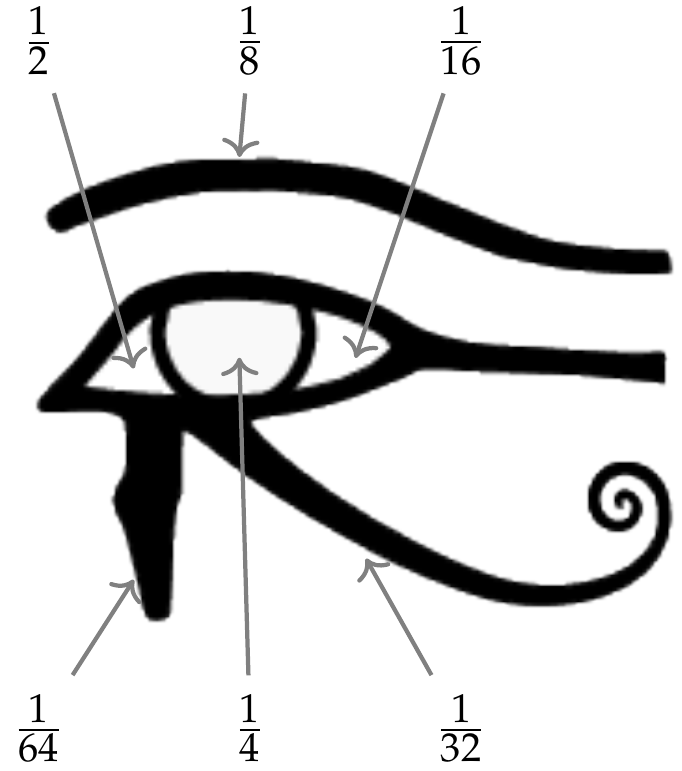
\includegraphics[alt=Figura: L'occhio di Horus.]{img/eyefra.png}
\else
  \immagine{Figura: L'occhio di Horus.}{\horus}
\fi
}

I Romani fecero poco uso dei numeri frazionari; si limitarono a considerare
le parti delle misure in uso che venivano divise in~12, 24, 36, 48\ldots 
Avevano pertanto simboli e nomi particolari per indicare alcune frazioni. 
\emph{Semis} per indicare~\(\frac{1}{2}\), il cui simbolo era~\(S\) 
oppure~\(Z\) 
\emph{sextans} per indicare~\(\frac{1}{6}\), \emph{dracma} per 
indicare~\(\frac{1}{96}\) e \emph{obolus} per indicare la sesta parte della 
\emph{dracma}.

Furono gli arabi a introdurre l'attuale scrittura delle
frazioni e i termini \emph{numeratore} e \emph{denominatore}.

La notazione attuale per le frazioni si deve sostanzialmente agli arabi, 
in Europa fu diffusa da Leonardo Pisano (Fibonacci) che nel il suo 
\emph{Liber Abaci} (1202) scrive e opera con le frazioni come oggi le 
conosciamo.

% ----------------------------------------------------------------------
\begin{comment}
\section{Frazioni}
\label{sec:03_frazioni}

\begin{definizione}{}{}
Una \emph{frazione} è una coppia ordinata di numeri naturali in cui il primo 
si chiama numeratore e il secondo denominatore. 
Il denominatore deve essere diverso da zero.
\end{definizione}

\begin{center}
 \input{\folder lbr/fig002_frazione.pgf}
\end{center}

Quando si chiede, per esempio un quarto di litro di 
latte,~\(\frac{1}{4}\munit{l}\), si danno le informazioni su come operare 
sulla grandezza unitaria litro per ottenere la quantità desiderata.
Le frazioni possono essere viste come operatori che si applicano a una 
grandezza fissata, considerata come l'intero o il tutto, per ottenere una 
nuova grandezza ben determinata e omogenea alla prima.

Una frazione con numeratore uguale a~1 è detta \emph{frazione unitaria}; 
indicata con~\(A\) una grandezza (segmento, peso, superficie, angolo\ldots) 
la scrittura~\(\frac{1}{n}A\) sta ad indicare l'operazione di divisione della 
grandezza~\(A\), intesa come il `tutto', in~\(n\) parti uguali.

Nella figura, il segmento unitario da~0 a~1 è stato diviso in due parti 
uguali 
ottenendo la frazione~\(\frac{1}{2}\)
dividendolo in quattro parti uguali si ottiene la frazione~\(\frac{1}{4}\)
dividendolo in otto parti uguali si ottiene la frazione~\(\frac{1}{8}\)
dividendolo in sedici parti uguali si ottiene la frazione~\(\frac{1}{16}\).

\begin{center}
 \input{\folder lbr/fig003_segmentounitario.pgf}
\end{center}

\begin{definizione}{}{}
Il \emph{denominatore} di una frazione è quel numero che indica in quante 
parti uguali si è diviso l'intero.
Poiché non ha senso dividere un intero in zero parti, il denominatore deve 
essere diverso da zero.
\end{definizione}

\begin{wrapfloat}{figure}{r}{0pt}
 \input{\folder lbr/fig004_quadrato.pgf}
\end{wrapfloat}

Vediamo un altro esempio. Il quadrato~\(Q\) della figura è stato diviso in 
quattro parti uguali e una parte è stata colorata di grigio; 
questa parte viene indicata con la frazione unitaria~\(\frac{1}{4}Q\).

Una frazione~\(\frac{1}{n}A\) significa l'ennesima parte di~\(A\), dove~\(A\) 
è 
il tutto che si deve dividere in~\(n\) parti uguali. In altre parole,
\(A\) si può ottenere moltiplicando per~\(n\) la frazione~\(\frac{1}{n}A\).

Partendo da~\(\frac{1}{n}A\) si possono considerare i suoi multipli interi:
\[\frac{2}{n}A, \frac{3}{n}A, \ldots, \frac{n}{n}A \] che rappresentano il
doppio di un ennesimo, il triplo di un ennesimo, l'intera grandezza~\(A\).

Riferendoci all'esempio del quadrato:
\begin{center}
 \input{\folder lbr/fig005_partiquadrati.pgf}
\end{center}

La frazione~\(\frac{m}{n}A\) (si legge \emph{emme ennesimi di}~\(A\)) con~\(m 
< 
n\) 
indica il multiplo secondo~\(m\) della frazione unitaria~\(\frac{1}{n}A\)
essa indica la grandezza che si ottiene dividendo~\(A\) in~\(n\) parti uguali 
e prendendone~\(m\).

\begin{definizione}{}{}
 Il \emph{numeratore} di una frazione è quel numero che esprime quante parti, 
 dell'intero suddiviso in parti secondo il denominatore, sono state prese.
\end{definizione}

Per leggere una frazione si legge prima il numeratore e poi il denominatore.
Quest'ultimo si legge come numero ordinale (terzo, quarto, quinto,\ldots) 
fino a~10 e se è maggiore di dieci si aggiunge la terminazione \emph{-esimo}.


\begin{esempio}{}{}
 Lettura di frazioni.
 \begin{htmulticols}{3}
 \begin{enumerate}[noitemsep, label=(\alph*)]
\item \(\dfrac{1}{2}\) si legge \emph{un mezzo};
\item \(\dfrac{1}{10}\) si legge \emph{un decimo};
\item \(\dfrac{2}{3}\), si legge \emph{due terzi};
\item \(\dfrac{1}{11}\) si legge \emph{un undicesimo};
\item \(\dfrac{5}{7}\) si legge \emph{cinque settimi};
\item \(\dfrac{1}{12}\) si legge \emph{un dodicesimo}.
\end{enumerate}
\end{htmulticols}
\end{esempio}


A volte per scrivere le frazioni si utilizza la scrittura del tipo~\(a/b\), 
quindi~\(2/3\)~\(4/6\)~\(6/9\)\ldots

\begin{definizione}{}{}
Si chiamano \emph{proprie} le frazioni che hanno il numeratore minore del 
denominatore.
Esse rappresentano sempre una grandezza minore dell'intero.
\end{definizione}

Vi sono frazioni che pur essendo formate da numeratori e denominatori 
diversi rappresentano la stessa parte dell'intero.
\begin{center}
 \input{\folder lbr/fig006_partintero.pgf}
\end{center}
%  \ovalbox{\risolvii \ref{ese:3.1}, \ref{ese:3.2}, \ref{ese:3.3}, 
\ref{ese:3.4}}

\begin{definizione}{}{}
Si dicono \emph{equivalenti} due frazioni che rappresentano la stessa parte 
dell'intero.
\end{definizione}

\begin{proprieta}[Invariantiva delle frazioni]
Se si moltiplica, o si divide, numeratore e denominatore di una stessa 
frazione per uno stesso numero diverso da zero si ottiene una frazione 
equivalente alla frazione data.
\end{proprieta}

Per trovare una frazione equivalente a una frazione assegnata è sufficiente 
moltiplicare per uno stesso numero il numeratore e il denominatore della 
frazione assegnata.


 \begin{esempio}{}{}
 Trovare due frazioni equivalenti a~\(\dfrac{4}{7}\).

Moltiplicando numeratore e denominatore per~2 si ha la frazione equivalente:
\[\frac{4\cdot2}{7\cdot2}=\frac{8}{14}.\]
Moltiplicando numeratore e denominatore per~3 si ha la frazione equivalente:
\[\frac{4\cdot3}{7\cdot3}=\frac{12}{21}.\]
 \end{esempio}


\begin{definizione}{}{}
Una frazione si dice \emph{ridotta ai minimi termini} se il numeratore e il 
denominatore sono due interi primi tra loro.
\end{definizione}

Per ridurre ai minimi termini una frazione occorre dividere numeratore e 
denominatore per il loro Massimo Comune Divisore.


 \begin{esempio}{}{}
Ridurre ai minimi termini la frazione~\(\dfrac{8}{12}\).

Scompongo in fattori~8 e~12, ottengo~\(8=2^3\) e~\(12=3\cdot2^2\).
Calcolo il~\(\mcd\) prendendo i fattori comuni con l'esponente più piccolo; 
in questo caso~\(2^2\) cioè~4. Divido numeratore e denominatore per~4:
\[\frac{8}{12} = \frac{8:4}{12:4} = \frac{2}{3}.\]
 \end{esempio}


Tutte le frazioni che hanno il denominatore (numero di parti in cui va divisa 
l'unità) uguale al numeratore (numero delle parti che vanno considerate) 
rappresentano l'intero:

\[\frac{2}{2}=\frac{3}{3}=\frac{10}{10}=1.\]

\begin{wrapfloat}{figure}{r}{0pt}
 \input{\folder lbr/fig011_interifraz.pgf}
\end{wrapfloat}

Per esempio, se divido un quadrato in due parti uguali e ne prendo due parti 
ottengo l'intero;
se divido un quadrato in tre parti uguali e ne prendo tre parti ottengo 
l'intero,\ldots

Cosa significa costruire la grandezza~\(\frac{6}{2}\) del quadrato~\(Q\)?
Tutte le frazioni che hanno il numeratore che è multiplo del denominatore 
rappresentano un multiplo dell'intero:
\[\frac{6}{2}=3,\qquad\frac{15}{3}=5,\qquad\frac{72}{6}=12.\]

\begin{definizione}{}{}
 Si chiamano \emph{apparenti} le frazioni che hanno il numeratore multiplo 
 del denominatore;
 esse rappresentano una grandezza multipla di quella presa come intero 
unitario.
\end{definizione}

Le frazioni che hanno il numeratore maggiore del denominatore rappresentano 
grandezze più grandi dell'intero.
Infatti le parti da considerare (indicate dal numeratore) sono di più delle 
parti in cui è divisa l'unità (indicate dal denominatore).
\begin{center}
 \input{\folder lbr/fig012_frazimpr.pgf}
\end{center}
\[\frac{5}{4}=\frac{4}{4}+\frac{1}{4}.\]

\begin{definizione}{}{}
 Si chiamano \emph{improprie} le frazioni che hanno il numeratore maggiore 
del 
 denominatore;
 esse rappresentano una grandezza maggiore della grandezza assegnata come 
intero.
\end{definizione}

% \ovalbox{\risolvii \ref{ese:3.5}, \ref{ese:3.6}, \ref{ese:3.7}, 
\ref{ese:3.8}, \ref{ese:3.9}, \ref{ese:3.10}, \ref{ese:3.11},
% \ref{ese:3.12}, \ref{ese:3.13}, \ref{ese:3.14}, \ref{ese:3.15}, 
\ref{ese:3.16}}

\section{Dalle frazioni ai numeri razionali}
\label{sec:03_razionali}

Abbiamo visto che ci sono delle frazioni che, pur essendo diverse tra di 
loro, 
rappresentano la stessa parte dell'intero: queste frazioni vengono chiamate 
\emph{frazioni equivalenti}.
Possiamo formare dei raggruppamenti di frazioni tra loro equivalenti, 
come nella figura \ref{fig:frazequiv}.

\begin{definizione}{}{}
Ogni raggruppamento di frazioni equivalenti è definito come un 
\emph{numero razionale assoluto} ed è rappresentato da una qualunque
frazione del raggruppamento; solitamente si sceglie la frazione ridotta ai 
minimi termini.
\end{definizione}

Nel nostro esempio~\(\frac{2}{3}\) è il numero razionale rappresentante del 
raggruppamento
\[\frac{2}{3}=\graffa\frac{2}{3}; \quad \frac{4}{6}; \quad \frac{6}{9}; 
\quad \frac{10}{15}; \quad \frac{14}{21}; \quad \ldots}.\]
In questo modo abbiamo dato al simbolo~\(a/b\) un nuovo significato, quello 
di 
numero e come tale la scrittura~\(a/b\) rappresenta il quoziente indicato tra 
i 
due numeri naturali~\(a\) e~\(b\). Scriveremo~\(2:3=~2/3\).

\begin{inaccessibleblock}[Figura: TODO]
 \begin{figure}[t]
\begin{center}
\input{\folder lbr/fig018_frazequiv.pgf}
\end{center}
\label{fig:frazequiv}
\caption{Esempi di frazioni equivalenti.}
\end{figure}
\end{inaccessibleblock}

\begin{definizione}{}{}
Un numero razionale assoluto preceduto dal segno è detto 
\emph{numero razionale}.
L'insieme dei numeri razionali relativi si indica con il simbolo~\(\insQ\).
\end{definizione}

Il segno del numero razionale relativo è quello che si ottiene dalla regola 
della
divisione dei segni tra numeratore e denominatore.


\begin{esempio}{}{}
Segno di numeri razionali.
\[\frac{-2}{-3}=+\frac{2}{3};\qquad\frac{2}{-3}=-\frac{2}{3};\qquad
\frac{-2}{3}=-\frac{2}{3}.\]
\end{esempio}


Le frazioni proprie, che hanno numeratore minore del denominatore, 
rappresentano sempre un numero compreso tra~0 e~1.

Le frazioni improprie, che hanno numeratore maggiore del denominatore, si 
possono scrivere come somma di un numero
naturale e di una frazione propria:

\begin{itemize} [noitemsep]
 \item il numero naturale è il risultato della divisione intera tra 
numeratore 
 e denominatore;
 \item il numeratore della frazione propria è il resto della divisione tra 
 numeratore e denominatore;
 \item il denominatore della frazione propria è il denominatore stesso della 
 frazione.
\end{itemize}

Le frazioni apparenti, del tipo
\(\frac{2}{2},\frac{6}{3},\frac{20}{5},\frac{12}{4},\frac{12}{3},\ldots\)
corrispondono a un numero intero, rispettivamente a~1, 2, 4, 3, 4.


 \begin{esempio}{}{}
 ~\(\dfrac{11}{3}=3+\dfrac{2}{3}\).
  \begin{itemize} [noitemsep]
   \item \(11 : 3 =~3\) il numero naturale;
   \item \(11\bmod~3 =~2\) numeratore della frazione propria;
   \item \(3 =\) denominatore della frazione propria.
  \end{itemize}
%\[\frac{11}{3}=3+\frac{2}{3}.\]
 \end{esempio}

 \begin{esempio}{}{}
 ~\(\dfrac{19}{7}=2+\dfrac{5}{7}\).
  \begin{itemize} [noitemsep]
   \item \(19 : 7 =~2\) il numero naturale;
   \item \(19\bmod~7 =~2\) numeratore della frazione propria;
   \item \(5 =\) denominatore della frazione propria.
  \end{itemize}
%\[\frac{19}{7}=2+\frac{5}{7}.\]
 \end{esempio}


% \ovalbox{\risolvii \ref{ese:3.17}, \ref{ese:3.18}}

\section{La scrittura dei numeri razionali}
\label{sec:03_decimali}

I numeri razionali, rappresentati finora come frazioni, possono essere 
scritti 
come numeri decimali:
basta fare la divisione tra numeratore e denominatore, il quoziente ottenuto 
è la rappresentazione della frazione sotto forma decimale.

\begin{center}
 \input{\folder lbr/fig019_raz.pgf}
\end{center}

I numeri decimali che si ottengono sono di due tipi: numeri decimali finiti 
come~\(1,375\) e numeri decimali periodici come~\(1,333333\ldots\)
quest'ultimo si scrive mettendo una barra sulla parte 
periodica:~\(1,\overline{3}\) oppure racchiudendo la parte periodica tra 
parentesi 
tonde~\(1,(3)\).

I numeri decimali finiti si ottengono dalle frazioni il cui denominatore ha 
come fattori solo il~2, solo il~5 o entrambi, eventualmente elevati a una 
potenza.

I numeri decimali periodici semplici si ottengono dalle frazioni il cui 
denominatore non ha per fattori né~2 né~5.

I numeri decimali periodici misti si ottengono dalle frazioni il cui 
denominatore contiene altri fattori oltre al~2 e al~5.


 \begin{esempio}{}{}
 Alcuni numeri decimali finiti.
\begin{enumerate}[noitemsep, label=(\alph*)]
 \item \(\dfrac{11}{8}=\dfrac{11}{2^3}=
\dfrac{11\cdot 5^3}{2^3\cdot 5^3}=\dfrac{1375}{1000}=1,375\)
 \item \(\dfrac{7}{25}=\dfrac{7}{5^2}=
\dfrac{7\cdot 2^2}{5^2\cdot 2^2}=\dfrac{28}{100}=0,28~\)
 \item \(\dfrac{13}{40}=\dfrac{13}{2^3\cdot 5}=
\dfrac{13\cdot 5^2}{2^3\cdot 5^3}=\dfrac{325}{1000}=0,325\)
 \item \(\dfrac{50}{7} = \dfrac{\ldots}{10}\), non è possibile, non è un 
 decimale finito.
\end{enumerate}
 \end{esempio}


% \ovalbox{\risolvi \ref{ese:3.19}}

\begin{procedura}{}{}
Trasformare una frazione in numero decimale:
\begin{enumerate}[noitemsep, label=(\alph*)]
 \item eseguire la divisione tra numeratore e denominatore;
 \item se la divisione ha un resto mettere la virgola al quoziente e 
 moltiplicare per~\(10\) il resto;
 \item continuare la divisione finché il resto è zero oppure fino a che non 
 si trova un resto già trovato prima;
 \item se la divisione si conclude con resto~\(0\) si ottiene un numero 
decimale 
 finito;
 \item se la divisione si conclude perché si è ritrovato un resto ottenuto in 
 precedenza si ottiene un numero decimale periodico.
\end{enumerate}
\end{procedura}

\clearpage


 \begin{esempio}{}{}
 Trasformazione di frazioni in numeri decimali.
  \begin{center}
  \input{\folder lbr/fig020_frazdec.pgf}
  \end{center}
  \begin{enumerate}[noitemsep, label=(\alph*)]
  \item \(\dfrac{113}{20}=5,65\), numero decimale finito;\vspace{1.03ex}
  \item \(\dfrac{17}{6}=2,8\overline{3}\), numero decimale periodico misto di 
  periodo~3;\vspace{1.03ex}
  \item \(\dfrac{15}{7}=2,\overline{142857}\), numero decimale periodico di 
  periodo~142857.
  \end{enumerate}
 \end{esempio}



% \ovalbox{\risolvi \ref{ese:3.20}, \ref{ese:3.21}}\vspazio

Viceversa un numero decimale finito o periodico può essere sempre scritto 
sotto forma di frazione.

\begin{procedura}{}{}
Trasformare un numero decimale finito in una frazione:
\begin{enumerate}[noitemsep, label=(\alph*)]
 \item scrivere una frazione che ha per numeratore il numero che si vuole 
  trasformare e per denominatore~uno;
 \item moltiplicare numeratore e denominatore per dieci elevato al numero
  di cifre a destra della virgola.
 \item semplificare la frazione così ottenuta.
\end{enumerate}
\end{procedura}

Per facilitare questa operazione possiamo considerare i numeri decimali 
finiti 
come frazioni particolari che hanno il numeratore uguale al numero decimale e 
il denominatore uguale a~1.


\begin{esempio}{}{}
Trovare la frazione equivalente a~1,36:
\[\frac{1,36}{1}=\frac{1,36\cdot10^2}{1\cdot10^2}=\frac{136}{100}=\frac{34}{25
}
.\].
\end{esempio}
\begin{esempio}{}{}
Trovare la frazione equivalente a~0,00043000:
\[\frac{0,00043}{1}=\frac{0,00043\cdot10^5}{1\cdot10^5}=\frac{43}{100000}.\]
\end{esempio}


Un numero decimale periodico, generalmente, presenta tre elementi:
\begin{description}
 \item [la parte intera] composta dalle cifre poste prima della virgola;
 \item [il periodo] che è composto da una o più cifre che si ripetono 
 all'infinito dopo la virgola;
 \item [l'antiperiodo] la parte composta da zero o più cifre  poste tra la 
 virgola e il periodo.
\end{description}


Per esempio, nel numero~253,485795795795795\ldots la parte intera è~253, 
il periodo è~579, l'antiperiodo è~48.

Dato che il numero è infinito non può essere scritto con tutte le sue cifre, 
si usano due modi per scriverlo in forma compatta, mettendo una lineetta 
sopra le cifre del periodo o racchiudendo le cifre del periodo tra parentesi 
tonde.

Il numero~253,485795795795795\ldots può essere 
scritto~\(253,48\overline{579}\), 
oppure~\(253,48(579)\).

I numeri decimali periodici si dividono in:
\begin{description}
 \item [semplici] se subito dopo la virgola è presente il periodo;
 \item [misti] se dopo la virgola è presente l'antiperiodo.
\end{description}

Anche i numeri periodici possono essere trasformati in una frazione, che si
dice \emph{frazione generatrice} del numero.

\begin{procedura}{}{}
 Determinare la frazione generatrice di un numero periodico:
\begin{enumerate}[noitemsep, label=(\alph*)]
 \item il numeratore della frazione si ottiene sottraendo dal numero 
  senza la virgola e con il periodo scritto una sola volta,
  il numero costituito dalle cifre che precedono il periodo;
 \item il denominatore della frazione si ottiene scrivendo tanti~\(9\) 
  quante sono le cifre del periodo seguiti da
  tanti~\(0\) quante sono le cifre comprese tra il periodo e la virgola;
 \item semplificare la frazione ottenuta.
\end{enumerate}
\end{procedura}

\paragraph*{Passo~\(a\)}~\(2,5\overline{12}\rightarrow~2512\).
\paragraph*{Passo~\(b\)}~\(2512-25=2487\).
\paragraph*{Passo~\(c\)}~\(2,5\overline{12}=\dfrac{2487}{990}\).


\paragraph*{Ma perché questa regola? Una possibile spiegazione}
Consideriamo il numero periodico semplice~\(2,\overline{3}\). Considero la 
frazione~\(\frac{2,\overline{3}}{1}\)
moltiplico numeratore e denominatore 
per~10~\(\frac{2,\overline{3}\cdot10}{1\cdot10}\) e ottengo
\(\frac{23,\overline{3}}{10}\).

L'obiettivo è quello di eliminare dal numeratore della frazione la parte 
decimale.
Per ottenere questo risultato tolgo~\(2,\overline{3}\) 
da~\(23,\overline{3}\), 
cioè \(23,\overline{3}-2,\overline{3}=21\).

Come mai~\(2,\overline{3}\) e non~\(1,\overline{3}\) o~\(0,\overline{3}\)?
Perché in questo modo posso sapere quanto vale il denominatore: 
se~\(23,\overline{3}\) è il risultato
della moltiplicazione di~\(2,\overline{3}\cdot10\),~\(21\)~è il risultato 
della moltiplicazione di
\(2,\overline{3}\cdot9\) in quanto~\(23,\overline{3}-2,\overline{3}=21\).
In definitiva
\[2,\overline{3}=\frac{23-2}{9}=\frac{21}{9}=\frac{7}{3}.\]

Possiamo usare lo stesso procedimento per il numero periodico 
misto~\(2,5\overline{12}\).

Considero la frazione~\(\frac{2,5\overline{12}}{1}\), moltiplico numeratore 
e denominatore per~1000 e ottengo: \(\frac{2512,\overline{12}}{1000}\).
L'obiettivo è quello di eliminare dal numeratore della frazione la parte 
decimale che contiene il periodo che si ripete all'infinito. 
Per ottenere questo risultato tolgo da~\(2512,\overline{12}\) questa volta
\(25,\overline{12}\), cioè~\(2512,\overline{12}-25,\overline{12}=2487\).
Per avere una frazione equivalente occorre che al denominatore abbia~990 in 
quanto dal numeratore ho tolto~10 volte \(2,5\overline{12}\).
\[2,5\overline{12}=\frac{2512-25}{990}=\frac{2487}{990}.\]

% \ovalbox{\risolvii \ref{ese:3.22}, \ref{ese:3.23}}

\subsection{Numeri periodici particolari}

Numeri periodici particolari sono quelli che hanno come periodo il numero~9,
come~\(2,\overline{9}\), \(1,1\overline{9}\), \(21,22\overline{9}\) ecc.
Se, per esempio, applichiamo la regola per il calcolo della frazione 
generatrice al numero periodico otteniamo un risultato inatteso
\[2,\overline{9}=\frac{29-2}{9}=\frac{27}{9}=3.\]
Quindi~\(2,\overline{9}\) coincide con il numero intero~3.

Per lo stesso motivo~\(1,1\overline{9}=1,2\),~\(21,22\overline{9}=21,23\).

\begin{wrapfloat}{figure}{r}{0pt}
\input{\folder lbr/fig021_perretre.pgf}
\end{wrapfloat}

Questo fatto si può anche dimostrare in modo grafico, rappresentando, 
ad esempio, il numero~\(0,\overline{9}\) e il numero~1 sulla retta reale.

Se i due numeri fossero veramente diversi sarebbero rappresentati da due 
punti 
distinti come in figura. Dato che la retta reale non può avere ``buchi'',
tra un suo punto e un altro ci deve essere almeno un altro numero compreso 
tra 
i due.
Ma qual è questo numero? Qualunque numero decimale minore di~1 è sicuramente 
superato dal numero~\(0,\overline{9}\),
ad esempio~0,9999999998 è sicuramente più piccolo di~\(0,\overline{9}\). 
Quindi non esiste nessun numero tra \(0,\overline{9}\) e~1,
di conseguenza i due numeri coincidono.

% \ovalbox{\risolvii \ref{ese:3.24}, \ref{ese:3.25}}



\section{I numeri razionali e la retta}
\label{sec:03_retta}

Anche i numeri razionali si possono rappresentare su una retta orientata. 
Per fare questo occorre scegliere un punto~\(O\) sulla retta e associare ad 
esso 
il numero zero. Fissiamo poi un segmento unitario e scegliamo un verso di 
percorrenza.

Dato un numero razionale positivo, rappresentato dalla 
frazione~\(\frac{a}{n}\), 
il punto corrispondente al numero razionale sulla retta viene determinato nel 
seguente modo. Dividiamo il segmento unitario~\(u\) in tante parti uguali
quante sono quelle indicate dal denominatore~\(n\) della frazione, ottenendo 
così la frazione unitaria~\(\frac{1}{n}\).
A partire dal punto~\(O\) procedendo verso destra, si contano~\(a\) frazioni 
unitarie. L'ultimo punto rappresenta il numero razionale~\(\frac{a}{n}\).

Per le frazioni improprie la singola unità~\(u\) non è sufficiente, occorre 
prendere la unità successiva di~\(u\) e dividere anche questa in~\(n\) parti. 
Il procedimento si ripete fino a che si considerano tutte le frazioni 
unitarie 
indicate da~\(a\). Anche in questo caso, il punto individuato dall'ultima 
frazione unitaria rappresenta il numero razionale~\(\frac{a}{n}\). 
In alternativa si può scomporre la frazione impropria nella somma di un 
numero 
intero e di una frazione propria, quindi si rappresenta la frazione impropria
a partire dal suo numero intero invece che partire da~0. Per esempio, per 
rappresentare la frazione~\(\frac{3}{2}\) trasformiamo la frazione 
in~\(1+\frac{1}{2}\), quindi rappresentiamo partendo dal numero~1 invece che 
da~0.

Se il numero razionale è negativo, ci comportiamo come prima con l'avvertenza 
di muoverci nel senso opposto a quello precedente cioè da destra verso 
sinistra.

\begin{center}
\input{\folder lbr/fig022_rettafraz.pgf}
\end{center}

% \ovalbox{\risolvii \ref{ese:3.26}, \ref{ese:3.27}, \ref{ese:3.28}}

\section{Confronto tra numeri razionali}
\label{sec:03_confronto}

Il numero razionale rappresentato dalla frazione~\(\frac{a}{n}\) è 
\emph{minore} 
del numero razionale rappresentato dalla frazione~\(\frac{b}{m}\), se nella 
retta orientata il punto che corrisponde alla frazione\(\frac{a}{n}\) precede 
il 
punto che corrisponde alla frazione\(\frac{b}{m}\) e si scrive
\[\frac{a}{n}<\frac{b}{m}.\]

Il numero razionale~\(\frac{a}{n}\) è \emph{maggiore} di~\(\frac{b}{m}\),
se nella retta orientata il punto che corrisponde alla 
frazione~\(\frac{a}{n}\) 
segue il punto che corrisponde alla frazione~\(\frac{b}{m}\) e si scrive
\[\frac{a}{n}>\frac{b}{m}.\]

Il numero razionale~\(\frac{a}{n}\) è \emph{equivalente} a~\(\frac{b}{m}\) se 
nella retta orientata i punti che corrispondono
alle frazioni~\(\frac{a}{n}\) e~\(\frac{b}{m}\) coincidono.

%% \newpage

\begin{esempio}{}{}
Confronto tra numeri razionali.
\begin{center}
\input{\folder lbr/fig022_rettafraz.pgf}
\end{center}
\[-\frac{13}{8}<-\frac{1}{2},\qquad\frac{3}{8}>-\frac{1}{2},\qquad
\frac{3}{8}<\frac{3}{2},\qquad-1>-\frac{13}{8}.\]
\end{esempio}


Per certe frazioni è facile vedere se una frazione precede o segue un'altra. 
Per altre non è così semplice.

Consideriamo per esempio le frazioni~\(\frac{7}{9}\) e~\(\frac{6}{7}\).
Quale frazione precede e quale segue? Il confronto non è immediato perché 
con la prima frazione si conta per unità frazionarie di tipo~\(\frac{1}{9}\), 
con la seconda per unità frazionarie di tipo~\(\frac{1}{7}\).

In generale, senza ricorrere alla rappresentazione sulla retta, come si 
possono confrontare i numeri razionali?

Conviene sostituire le frazioni date con altre equivalenti che hanno unità 
frazionarie dello stesso tipo:
cioè occorre ridurre le frazioni allo stesso denominatore.

\begin{procedura}{}{}
Confrontare due frazioni:
\begin{enumerate}[noitemsep, label=(\alph*)]
\item si calcola il minimo comune multiplo dei denominatori delle frazioni;
\item si trasforma ciascuna frazione come segue:
\begin{itemize} [noitemsep]
\item il nuovo denominatore è il~\(\mcm\) trovato;
\item il nuovo numeratore si ottiene dividendo il~\(\mcm\) per il 
denominatore della frazione data e moltiplicando il quoziente ottenuto per il 
numeratore della frazione data.
\end{itemize}
\item si confrontano i nuovi numeratori: la frazione più grande è quella che 
ha il numeratore più grande.
\end{enumerate}
\end{procedura}

Un altro modo per confrontare due frazioni consiste nel 
\emph{moltiplicare in croce} numeratori e denominatori delle frazioni, 
come nei seguenti esempi.


\begin{esempio}{}{}
Confronta~\(\frac{3}{2}\) con~\(\frac{5}{3}\).

Moltiplichiamo il numeratore della prima frazione con il denominatore della 
seconda frazione e il denominatore della prima frazione per il denominatore 
della seconda, così:
 \[\frac{3}{2}<\frac{5}{3}\text{, perché }3\cdot3<2\cdot5. \]
\end{esempio}

\begin{esempio}{}{}
Confronta le frazioni~\(\frac{7}{9}\) e~\(\frac{6}{7}\).

\(\mcm(7.9)=63\).
\[\frac{7}{9}=\frac{7\cdot7}{9\cdot7}=\frac{49}{63},\qquad%
\frac{6}{7}=\frac{6\cdot9}{7\cdot9}=\frac{54}{63}.\]
\[\frac{54}{63}>\frac{49}{63}\Rightarrow\frac{6}{7}>\frac{7}{9}.\]
\end{esempio}


% \ovalbox{\risolvii \ref{ese:3.29}, \ref{ese:3.30}, \ref{ese:3.31}, 
\ref{ese:3.32}, \ref{ese:3.33}, \ref{ese:3.34}, \ref{ese:3.35}, 
\ref{ese:3.36}, 
\ref{ese:3.37}, \ref{ese:3.38},%
% \ref{ese:3.39}, \ref{ese:3.40}, \ref{ese:3.41},}

% \vspazio\ovalbox{\ref{ese:3.42}, \ref{ese:3.43}}

\section{Le operazioni con i numeri razionali}
\label{sec:03_operazioni}

Con i numeri razionali è sempre possibile eseguire le addizioni, 
le moltiplicazioni, le sottrazioni e le divisioni.
In altre parole, poiché un numero razionale può essere scritto sotto forma 
di frazione, se si addizionano,
si moltiplicano, si sottraggono, si dividono due frazioni il risultato è 
sempre una frazione.

\subsection{Addizione}

Se due frazioni hanno la stessa unità frazionaria allora è sufficiente 
sommare 
i numeratori delle frazioni e prendere come denominatore l'unità frazionaria 
comune.
\[\frac{5}{3}+\frac{2}{3}=\frac{5+2}{3}=\frac{7}{3}.\]
%
%\begin{center}
%\input{\folder lbr/fig024_addi.pgf}
%\end{center}

\begin{definizione}{}{}
La \emph{somma di due frazioni con lo stesso denominatore} è una frazione che 
ha per denominatore lo stesso denominatore delle frazioni date e per 
numeratore la somma dei numeratori.
\end{definizione}


Se le unità frazionarie sono diverse dobbiamo considerare frazioni 
equivalenti 
a quelle date che abbiano la stessa unità frazionaria e poi eseguire 
l'addizione come indicato nel punto precedente e cioè sommando i numeratori 
e lasciando lo stesso denominatore comune.

\begin{center}
\input{\folder lbr/fig025_addii.pgf}
\end{center}

In generale data l'addizione di due frazioni~\(\frac{m}{n}+\frac{p}{q}\) la 
somma si può scrivere come
\[\frac{mq +pn}{nq}.\]

\begin{center}
\input{\folder lbr/fig026_addiii.pgf}
\end{center}

Quando si sommano due frazioni si può scegliere un qualsiasi denominatore 
comune, tuttavia per semplificare i calcoli conviene scegliere il più piccolo 
possibile, cioè il minimo comune multiplo dei denominatori delle frazioni da 
sommare.

\begin{procedura}{}{}
Sommare due o più frazioni:
\begin{enumerate}[noitemsep, label=(\alph*)]
\item ridurre le frazioni ai minimi termini;
\item calcolare il~\(\mcm\) dei denominatori;
\item mettere il~\(\mcm\) come denominatore della frazione somma;
\item per ogni frazione dividere il~\(\mcm\) per il suo denominatore e 
moltiplicare il risultato per il numeratore della frazione mantenendo il 
segno;
\item calcolare la somma algebrica di tutti i numeri trovati;
\item mettere la somma ottenuta come numeratore della frazione somma;
\item ridurre ai minimi termini la frazione ottenuta.
\end{enumerate}
\end{procedura}


\begin{esempio}{}{}
Sommare le frazioni~\(\frac{8}{12}- \frac{5}{6}+\frac{8}{5}-1\).

\paragraph*{Passo~\(a\)} riduco ai minimi termini le frazioni
\(\displaystyle{\frac{2}{3}-\frac{5}{6}+\frac{8}{5}-\frac{1}{1}}\)
\paragraph*{Passo~\(b\)} calcolo~\(\mcm(3,6,5,1)=30\).
\paragraph*{Passo~\(c\)} la frazione somma avrà come denominatore il~\(\mcm\) 
trovato~\(\dfrac{\ldots}{30}\).
\paragraph*{Passo~\(d\)} per ogni frazione divido il~\(\mcm\) per il suo 
denominatore e moltiplico il risultato per il numeratore:
\begin{align*}
\frac{2\cdot(30:3)-5\cdot(30:6)+8\cdot(30:5)-1\cdot(30:1)}{30}&=
\frac{2\cdot10-5\cdot5+8\cdot6-1\cdot30}{30}\\
&=\frac{20-25+48-30}{30}.
\end{align*}

\paragraph*{Passo~\(e\)} calcolo la somma algebrica dei numeri ottenuti al 
numeratore~\(+13\).
\paragraph*{Passo~\(f\)} metto la somma ottenuta al numeratore della frazione 
somma~\(+\dfrac{13}{30}\).
\paragraph*{Passo~\(g\)} vedo se posso ridurre la frazione, in questo caso 
no, 
il risultato è~\(+\dfrac{13}{30}\).
\end{esempio}

\begin{esempio}{}{}
Sommare i numeri razionali~\(-0,2-1,\overline{2}+25\%+\frac{7}{12}\).

Trasformo i numeri razionali in frazioni:
\[-\frac{2}{10}-\frac{12-1}{9}+\frac{25}{100}+\frac{7}{12}=-\frac{1}{5}-
\frac{11}{9}+\frac{1}{4}+\frac{7}{12}.\]

Quindi~\(\mcm(5,9,4,12)=180\).

\begin{align*}
\frac{-1\cdot(180:5)-11\cdot(180:9)+1\cdot(180:4)+7\cdot(180:12)}{180}&=
\frac{-1\cdot36-11\cdot20+1\cdot45+7\cdot15}{180}\\
&=\frac{-36-220+45+105}{180}\\
&=-\frac{106}{180} \\
&=-\frac{53}{90}.
\end{align*}
\end{esempio}


\subsection{Sottrazione di frazioni}

La sottrazione di frazioni si può sempre trasformare in una addizione tra la 
prima frazione e l'opposto della seconda frazione. 
Come per i numeri relativi, quando si parla di somma di frazioni si intende 
sempre somma algebrica di frazioni.

% \vspazio\ovalbox{\risolvii \ref{ese:3.44}, \ref{ese:3.45}, \ref{ese:3.46}, 
\ref{ese:3.47}}

\subsection{Moltiplicazione}

Il risultato della moltiplicazione tra frazioni può essere interpretato come 
l'area di un rettangolo in cui le frazioni fattori sono la base e l'altezza.
\begin{center}
 \input{\folder lbr/fig027_frazmol.pgf}
\end{center}

Moltiplicare~\(\frac{4}{5}\cdot\frac{2}{3}\) è come calcolare l'area del 
rettangolo di base~\(\frac{4}{5}\) e altezza \(\frac{2}{3}\). 
Ogni rettangolino di base~\(\frac{1}{5}\) e altezza~\(\frac{1}{3}\) ha 
area~\(\frac{1}{15}\).
I rettangolini da prendere in considerazione sono~8. Il risultato è 
quindi~\(\frac{8}{15}\). 
Il denominatore indica in quante parti è stato diviso il quadrato unitario: 
sono \(3 \cdot 5=15\) parti.
Il numeratore indica quante parti prendiamo, sono le parti \(2\cdot 4=8\) in 
grigio. 

Il prodotto di due frazioni è una frazione che ha per numeratore il prodotto 
dei numeratori e per denominatore il prodotto dei denominatori.

\begin{center}
 \input{\folder lbr/fig028_frazmol.pgf}
\end{center}

% \ovalbox{\risolvii \ref{ese:3.48}, \ref{ese:3.49}, \ref{ese:3.50}, 
\ref{ese:3.51}}

\subsection{Operazione inversa e aritmetica dell'orologio}

La divisione è l'operazione inversa della moltiplicazione. 
Ma cosa significa operazione inversa?
Una operazione può essere interpretata come qualsiasi azione che provoca 
un cambiamento di stato.

Consideriamo come esempio l'addizione nell'orologio che segna le ore 
dodici~\((12 =~0)\).
Addizionare significa spostare le lancette in avanti di un determinato 
numero di ore.
Si riporta la tabella dell'addizione dell'orologio.

Consideriamo l'addizione~\(9+7=4\).
Il primo elemento~9 può essere interpretato come stato iniziale,~\(+~7\) 
come operatore formato dall'operazione 
<<spostare le lancette avanti di\ldots>> e dall'argomento~7; 
il risultato~4 è lo stato finale.

Si indica come operazione inversa quella operazione che applicata allo stato 
finale con argomento uguale a quello precedente dell'operazione diretta, 
riporta allo stato iniziale.

Notiamo che anche nella matematica dell'orologio l'addizione gode della 
proprietà commutativa e associativa, ha l'elemento neutro che è~0, 
ogni numero ha l'inverso.

\begin{center}
 \input{\folder lbr/fig029_aritoro.pgf}
\end{center}

\begin{htmulticols}{2}
\begin{itemize} [noitemsep]
\item L'inverso di~0 è~0 perché~\(0+0=0\)
\item l'inverso di~1 è~11 perché~\(1+11=0\)
\item l'inverso di~2 è~10 perché~\(2+10=0\)
\item l'inverso di~3 è~9 perché~\(3+9=0\)
\item l'inverso di~4 è~8 perché~\(4+8=0\)
\item l'inverso di~5 è~7 perché~\(5+7=0\).
\end{itemize}
\end{htmulticols}

L'elemento inverso è molto importante in quanto ci permette di sostituire 
l'operazione inversa, con l'operazione diretta che ha come argomento 
l'elemento inverso dell'argomento dell'operazione diretta.
%% \newpage
\begin{center}
 \input{\folder lbr/fig030_orol.pgf}
\end{center}

Così per tornare allo stato iniziale invece di operare con portare 
indietro le lancette di~7, otteniamo lo stesso risultato portando avanti 
le lancette di~5 che è appunto l'inverso di~7.

\subsection{Divisione}

La divisione è l'operazione inversa della moltiplicazione.
Dato che nell'insieme dei numeri razionali esiste sempre l'inverso di una 
frazione rispetto alla moltiplicazione, esclusa la frazione zero, si può 
sempre eseguire la divisione di due qualsiasi frazioni.

\begin{center}
 \input{\folder lbr/fig031_divisione.pgf}
\end{center}

\[\frac{m}{n}:\frac{p}{q}=\frac{m}{n}\cdot\frac{q}{p}=\frac{mq}{np}.\]

Il quoziente di due frazioni è la frazione che si ottiene moltiplicando la 
prima frazione per l'inverso della seconda frazione.


 \begin{esempio}{}{}
Quoziente di due frazioni.
\begin{itemize} [noitemsep]
\item \(\displaystyle{\frac{2}{3}:\frac{7}{4}}\).
\end{itemize}
Il reciproco di~\(\frac{7}{4}\) è~\(\frac{4}{7}\). Pertanto
\[\frac{2}{3}:\frac{7}{4}\rightarrow\frac{2}{3}\cdot\frac{4}{7}=\frac{8}{21}.\
]

\begin{itemize} [noitemsep]
	\item \(\displaystyle{-\frac{2}{3}:\tonda{-\frac{3}{4}}}\).
\end{itemize}
Il reciproco di~\(-\frac{3}{4}\) è~\(-\frac{4}{3}\). Pertanto
\[-\frac{2}{3}:\tonda{-\frac{3}{4}}\rightarrow-\frac{2}{3}\cdot
\tonda{-\frac{4}{3}}=+\frac{8}{9}.\]

\begin{itemize} [noitemsep]
 \item \(\displaystyle{\frac{2}{3}:0}\).
\end{itemize}
 Il reciproco di~0 non esiste, quindi la divisione non è eseguibile.

\begin{itemize} [noitemsep]
 \item \(0:\dfrac{2}{3}\).
\end{itemize}
Il reciproco di~\(\frac{2}{3}\) è~\(\frac{3}{2}\). Pertanto
\[0:\frac{2}{3}\rightarrow~0\cdot \frac{3}{2}=0.\]
\end{esempio}


% \ovalbox{\risolvii \ref{ese:3.52}, \ref{ese:3.53}, \ref{ese:3.54}, 
\ref{ese:3.55}}

\section{Potenza di una frazione}
\label{sec:03_potenza}

Come per ogni numero, anche per le frazioni, la potenza di una frazione non è
altro che un prodotto di tante frazioni identiche alla frazione data quanto è 
il valore dell'esponente, pertanto si trova elevando il numeratore e il 
denominatore della frazione all'esponente della potenza.
\[\tonda{\frac{a}{b}}^n=\underbrace{\frac{a}{b}\cdot\frac{a}{b}\cdot
\frac{a}{b}\cdot\ldots\cdot\frac{a}{b}}_%
{n\text{ volte}}=\frac{a^n}{b^n}.\]


\begin{esempio}{}{}
Potenza di frazioni.
\begin{htmulticols}{3}
\begin{itemize} [noitemsep]
\item \(\displaystyle{\tonda{-\frac{2}{3}}^3=-\frac{8}{27}}\)
\item \(\displaystyle{-\frac{2^3}{3}=-\frac{8}{3}}\)
\item \(\displaystyle{\tonda{-\frac{2}{3}}^2=+\frac{4}{9}}\).
\end{itemize}
\end{htmulticols}
\end{esempio}


\subsection{Potenza con esponente uguale a zero}
La definizione di potenza si estende anche al caso in cui l'esponente è zero.

Consideriamo l'esempio della divisione di due potenze con la stessa base e 
con 
lo stesso esponente:
\begin{itemize} [noitemsep]
\item \(a^n:a^n=1\), la divisione di due numeri uguali è~1;
\item \(a^n:a^n=a^0\), applicando le proprietà delle potenze.
\end{itemize}

Possiamo allora concludere che per ogni frazione o numero razionale~\(a\) 
diverso da zero~\(a^0=1\). Non è invece possibile la potenza~\(0^0\).

\subsection{Potenza con esponente un numero intero negativo}

La definizione di potenza si può estendere anche al caso in cui l'esponente 
sia uguale a un numero intero negativo:
\[a^{-n}=a^0:a^n=1:a^n=\frac{1}{a^n}=\frac{1^n}{a^n}=\tonda{\frac{1}{a}}^
n
.\
]

Si può definire allora per ogni numero razionale diverso da zero
\[a^{-n}=\tonda{\frac{1}{a}}^n.\]

La potenza di un numero diverso da zero elevato a un esponente intero 
negativo 
è uguale a una potenza che ha per base il reciproco della base rispetto
alla moltiplicazione e per esponente l'opposto dell'esponente rispetto 
all'addizione.

Non è definita invece la potenza con esponente negativo di~0. Il numero~0 
infatti non ha il reciproco. 
Pertanto,~\(0^{-n}\) è una scrittura priva di significato.

% \vspazio\ovalbox{\risolvii \ref{ese:3.56}, \ref{ese:3.57}, \ref{ese:3.58}, 
\ref{ese:3.59}, \ref{ese:3.60}}

\section{Notazione scientifica e ordine di grandezza}
\label{sec:03_ordinedigrandezza}

\section{Le percentuali}
\label{sec:03_percentuali}

Avrai sentito parlare spesso che il prezzo di un oggetto è stato scontato 
del~10 per cento, oppure che un partito politico ha preso il~25 per cento di 
voti e altre espressioni simili che coinvolgono le percentuali.

Le percentuali sono un altro modo per scrivere le frazioni.

\begin{definizione}{}{}
Le \emph{percentuali} sono frazioni che hanno come denominatore~100 e come 
numeratore un numero intero o decimale.
\end{definizione}

La percentuale si indica con un numero intero o decimale seguita dal simbolo 
\%.
\[35\%=\frac{35}{100};\qquad7\%=\frac{7}{100};\qquad~12,5\%=\frac{12,5}{100}=
\frac{125}{1000}.\]

Per passare dalla scrittura percentuale alla scrittura decimale basta 
dividere 
per~100 il numero che esprime la percentuale:
\[35\%=\frac{35}{100}=0,35;\qquad7\%=\frac{7}{100}=0,07;\qquad12,5\%=
\frac{12,5}{100}=0,125.\]

Per passare dalla scrittura decimale alla scrittura in percentuale basta 
moltiplicare numeratore e denominatore per~100:
\[0,02=\frac{0,02}{1}=\frac{2}{100}=2\%;\qquad0,23=\frac{0,23}{1}=
\frac{23}{100}=23\%; \qquad1,21=\frac{1,21}{1}=\frac{121}{100}=121\%.\]

Per passare da una frazione alla percentuale conviene prima scrivere la 
frazione come numero decimale e poi da questo passare alla percentuale:
\[\frac{2}{3}=0,\overline{6}=\frac{0,\overline{6}}{1}=\frac{66,\overline{6}}{
100
}=66,
\overline{6}\%.\]

% \vspazio\ovalbox{\risolvii \ref{ese:3.79}, \ref{ese:3.80}, \ref{ese:3.81}, 
\ref{ese:3.82}}

\subsection{Problemi con le percentuali}

Per calcolare la percentuale di una grandezza è sufficiente moltiplicare il 
valore della grandezza per la percentuale espressa in frazione.


 \begin{esempio}{}{}
In una scuola che ha~857 alunni ne sono stati promossi il~95\%. 
Quanti sono stati i promossi?

Per rispondere, si moltiplica il numero totale di alunni per la 
frazione~\(95/100\).
Precisamente~\(\frac{95}{100}\cdot857=814,15\).
Poiché il risultato non è un numero intero la percentuale è stata 
approssimata. Gli alunni promossi sono stati~814.
 \end{esempio}


A volte è nota una parte della grandezza e si vuole conoscere che percentuale 
è
la parte nota rispetto al totale. In questo caso occorre dividere la parte 
nota per l'intera grandezza, moltiplicare il risultato per~100 ed esprimere 
il numero in percentuale.


\begin{esempio}{}{}
Di una scolaresca di~652 alunni ben~126 hanno avuto il debito in matematica.
Qual è la percentuale di alunni che hanno avuto il debito in matematica?

Per rispondere alla domanda eseguiamo i seguenti calcoli:
\[\frac{126}{652}\cdot100\%\approx0,19\cdot100\%=19\%.\]
\end{esempio}


\subsection{Problemi con gli sconti}


 \begin{esempio}{}{}
Un pantalone costava \officialeuro\ 70 e viene venduto con il~\(20\%\) di 
sconto, 
a quanto viene venduto?

Si tratta di calcolare prima lo sconto e po il prezzo scontato. 
Lo sconto è dato da

\begin{center}
\(\displaystyle{20\%\cdot70}\) \officialeuro\ \(=\dfrac{20}{100}\cdot70\) 
\officialeuro\ \(=14\).
\end{center}

Il prezzo scontato è \officialeuro\ \(70 -\) \officialeuro\ 14~\(=\) 
\officialeuro\ 56.

In alternativa si può tenere conto che, se~\(20\%\) esprime lo sconto, la 
parte 
rimanente, quella da pagare, è \(100\%-20\%=80\%\). 
Quindi per calcolare quanto costano i pantaloni scontati si può calcolare

\begin{center}
\(\displaystyle{80\%\cdot70}\) \officialeuro\ \(=\dfrac{80}{100}\cdot70\) 
\officialeuro\ \(=56\) \officialeuro.
 \end{center}
 \end{esempio}

 \begin{esempio}{}{}
Un paio di scarpe da \officialeuro\ 120 viene venduto scontato a 
\officialeuro\ 75 Qual è stata la percentuale di sconto praticato?

Per rispondere alla domanda, calcolo lo sconto \officialeuro\ 120~\(-\) 
\officialeuro\ 75~\(=\) \officialeuro\ 45.

Calcolo la percentuale che \officialeuro\ 45 rappresentano di 
\officialeuro\ 120, \[\frac{45}{120}\cdot100\%=0,375\cdot100\% =~37,5\%.\]
 \end{esempio}

\begin{esempio}{}{}
Mario ha trovato in un negozio il computer che stava cercando; per fortuna 
era scontato del~\(15\%\), ha risparmiato cosi~120 euro. 
Quanto costa il computer di listino?

\officialeuro\ 120 corrispondono al~\(15\%\) del prezzo di listino.
Per calcolare il prezzo di listino occorre dividere~120 per la frazione 
che corrisponde a~\(15\%\).
\begin{center}
 \(120:~15\% =~120:\dfrac{15}{100} =120\cdot\dfrac{100}{15}=\) \officialeuro\ 
800.
\end{center}
\end{esempio}



% \ovalbox{\risolvii \ref{ese:3.83}, \ref{ese:3.84}, \ref{ese:3.85}, 
% \ref{ese:3.86}, \ref{ese:3.87},
% \ref{ese:3.88}, \ref{ese:3.89}, \ref{ese:3.90}, \ref{ese:3.91}, 
% \ref{ese:3.92}, \ref{ese:3.93},
% \ref{ese:3.94}, \ref{ese:3.95},}

% \vspazio\ovalbox{\ref{ese:3.96}, \ref{ese:3.97}, \ref{ese:3.98}, 
% \ref{ese:3.99}, \ref{ese:3.100}, \ref{ese:3.101},
% \ref{ese:3.102}, \ref{ese:3.103}, \ref{ese:3.104}, \ref{ese:3.105}, 
% \ref{ese:3.106}, \ref{ese:3.107}, \ref{ese:3.108},
% \ref{ese:3.109},}
% 
% \vspazio\ovalbox{\ref{ese:3.110}, \ref{ese:3.111}, \ref{ese:3.112}, 
% \ref{ese:3.113}, \ref{ese:3.114}}

\section{Proporzioni}
\label{sec:03_proporzioni}

\begin{definizione}{}{}
Il rapporto tra due numeri, di cui il secondo è diverso da zero, è il 
quoziente che si ottiene dividendo il primo numero per il secondo. 
Il primo numero si dice \emph{antecedente}, il secondo \emph{conseguente}.
\end{definizione}

\begin{center}
  \input{\folder lbr/fig033_antecons.pgf}
\end{center}

\begin{definizione}{}{}
 Una \emph{proporzione} è una uguaglianza tra due rapporti, del tipo
\[A: B = C: D,\]
che si legge \emph{\(A\) sta a~\(B\) come~\(C\) sta a~\(D\)}, con~\(B\) 
e~\(D\) 
diversi da 
zero.
\end{definizione}

\begin{center}
  \input{\folder lbr/fig034_propor.pgf}
\end{center}


 \begin{esempio}{}{}
  \(4:~2 =~12:~6\).

Formano una proporzione perché i due quozienti valgono entrambi~2.
 \end{esempio}

\begin{esempio}{}{}
\(7:~14 =~16:~4\).

 \emph{Non} formano una proporzione perché il primo rapporto vale~0,5 mentre 
 il secondo rapporto vale~4.
\end{esempio}


Si dice anche che quattro numeri sono in proporzione se il rapporto tra i 
primi due è uguale al rapporto tra il terzo e il quarto.
 
\begin{proprieta}[Fondamentale delle proporzioni]
  In ogni proporzione il prodotto dei medi è uguale al prodotto degli estremi.
\[A:B=C:D\Rightarrow A\cdot D=B\cdot C.\]
\end{proprieta}


 \begin{esempio}{}{}
\(4:~6 =~6:~9\).

Il prodotto dei medi è~\(6\cdot6=36\) e il prodotto degli estremi 
è~\(4\cdot9=36\). 
Quindi è una proporzione.
 \end{esempio}

\begin{esempio}{}{}
\(20:~30 =~30:~40\).

Il prodotto dei medi è~\(30\cdot30=900\) il prodotto degli estremi 
è~\(20\cdot40=800\). Quindi non è una proporzione.
\end{esempio}


% \begin{proprieta}[del permutare]
% Se in una proporzione scambiamo tra di loro i medi otteniamo ancora una 
% proporzione; in modo analogo otteniamo ancora una proporzione se scambiamo 
% tra di loro gli estremi, o ancora se scambiamo tra di loro sia i medi sia 
% gli estremi.
% \[A: B = C: D\Rightarrow A: C = B: D\Rightarrow D: B = C: A\Rightarrow 
% D: C = B: A.\]
% \end{proprieta}
% 
% 
%  \begin{esempio}{}{}
% Data la proporzione~\(12:~16 =~18:~24\) e scambiando tra di loro:
% \begin{itemize} [noitemsep]
%   \item i medi si ottiene la proporzione~\(12:~18 =~16:~24\)
%   \item gli estremi si ottiene la proporzione~\(24:~16 =~18:~12\)
%   \item sia i medi sia gli estremi si ottiene la 
%     proporzione~\(24:~18 =~16:~12\).
% \end{itemize}
% 
%  \end{esempio}
% 
% 
% 
% \begin{proprieta}[dell'invertire]
%   Se in una proporzione scambiamo ogni antecedente con il rispettivo 
%   conseguente
% otteniamo ancora una proporzione.
% \[A: B = C: D\Rightarrow B: A = D: C.\]
% \end{proprieta}
% 
% 
%  \begin{esempio}{}{}
% Data la proporzione~\(15:~9 =~5:~3\), applicando la proprietà dell'invertire
% otteniamo la proporzione~\(9:~15 =~3:~5\).
%  \end{esempio}
% 
% 
% \begin{proprieta}[del comporre]
% In una proporzione la somma dei primi due termini sta al primo termine come 
% la somma del terzo e del quarto termine sta al terzo termine. Analogamente,
% la somma dei primi due termini sta al secondo termine come la somma del 
% terzo e del quarto termine sta al quarto termine.
% \[A: B = C: D\Rightarrow (A+B): A = (C+D): C.\]
% \[A: B = C: D\Rightarrow (A+B): B = (C+D): D.\]
% \end{proprieta}
% 
% 
%  \begin{esempio}{}{}
% Data la proporzione~\(16:~10 =~40:~25\), applicando la proprietà del 
comporre 
% si ottengono le proporzioni
% \[26:~16 =~65:~40,\qquad26:~10 =~65:~25.\]
%  \end{esempio}
% 
% 
% Analogamente alla proprietà del comporre si ha la seguente:
% 
% \begin{proprieta}[dello scomporre]
%   In una proporzione la differenza dei primi due termini sta al primo 
% termine come la differenza del
% terzo e del quarto termine sta al terzo termine. Analogamente, la 
differenza 
% dei primi due termini % sta al secondo termine come la differenza del terzo 
% e del quarto termine sta al quarto termine.
% \[A: B = C: D\Rightarrow (A-B): A = (C-D): C.\]
% \[A: B = C: D\Rightarrow (A-B): B = (C-D): D.\]
% \end{proprieta}
% 
% 
%  \begin{esempio}{}{}
% Data la proporzione~\(16:~10 =~40:~25\), applicando la proprietà dello 
scomporre 
% si ottengono le proporzioni
% \[6:~16 =~15:~40,\qquad6:~10 =~15:~25.\]
%  \end{esempio}
% 

\subsection{Calcolo di un medio o un estremo incognito}
Il medio incognito di una proporzione si calcola moltiplicando gli estremi e 
dividendo il risultato per l'altro medio:
\[a:b=x:d\Rightarrow x=\frac{a\cdot d}{b}.\]

L'estremo incognito di una proporzione si calcola moltiplicando i medi e 
dividendo il risultato per l'altro estremo:
\[x:b=c:d\Rightarrow x=\frac{b\cdot c}{d}.\]

\vspace{-1ex}
\begin{esempio}{}{}
Calcola il termine incognito di ciascuna proporzione.
\vspace{-1.3ex}\begin{itemize} [noitemsep]
  \item \(5:7=20:x\Rightarrow x=\frac{7\cdot 20}{5}=28\)
  \item \(2:x=~3:16\Rightarrow x=\frac{2\cdot 16}{3}=\frac{32}{3}\)
  \item \(\frac{2}{3}:\frac{1}{2}=x:\frac{5}{6}%
\Rightarrow x=\frac{2}{3}\cdot\frac{5}{6}:\frac{1}{2}=\frac{2}{3}%
\cdot\frac{5}{6}\cdot\frac{2}{1}=\frac{10}{9}\).
\end{itemize}
\end{esempio}%\vspace*{-1.7ex}


\begin{definizione}{}{}
  Una proporzione si dice \emph{continua} se ha i medi uguali.
\end{definizione}

Una proporzione continua è del tipo~\(A: B = B: C\), per esempio
\[3:~9 =~9:~27,\qquad5:~10 =~10:~20,\qquad4:~16 =~16:~64.\]

\subsubsection*{Calcolo del medio in una proporzione continua}

In una proporzione continua il medio proporzionale incognito si ottiene 
moltiplicando gli estremi e calcolando la radice quadrata del prodotto 
ottenuto.
\[a:x=x:d\Rightarrow x=\sqrt{a\cdot d}.\]


\begin{esempio}{}{}
Trovare il valore di x nella seguente proporzione continua~\(36: x = x:~9\).

Svolgimento~\(x=\sqrt{36\cdot 9}=18\).
\end{esempio}


% \subsubsection*{Calcolo di un termine incognito per mezzo delle proprietà 
del 
% comporre e dello scomporre}
% 
% 
%   \begin{esempio}{}{}
%     \((11-x): x =~15:~5\).
% 
%   Applicando la proprietà del comporre si ha la proporzione
%   \begin{align*}
%   (11-x+x): x = (15+5):~5 &\Rightarrow~11:x=20:5\\
%   &\Rightarrow x=\frac{11\cdot5}{20}=\frac{11}{4}.
%   \end{align*}
%   \end{esempio}
% 
% \begin{esempio}{}{}
%  ~\(\displaystyle{\tonda{\frac{1}{2}+x}:\frac{5}{8}=x:5}\).
% 
%  Permutando i medi si ha~\(\displaystyle{\tonda{\frac{1}{2}+x}:x=
% \frac{5}{8}:5}\). Applicando la proprietà
% dello scomporre si ha:
% \begin{align*}
%   &\tonda{\frac{1}{2}+x-x}:x=\tonda{\frac{5}{8}-5}:5\\
% \Rightarrow &\frac{1}{2}:x=\frac{-35}{8}:5\\
% \Rightarrow 
&x=\frac{1}{2}\cdot5:\tonda{\frac{-35}{8}}=\frac{1}{2}\cdot5%
% \cdot\tonda{-\frac{8}{35}}=-\frac{4}{7}.
% \end{align*}
% \end{esempio}
% 


% % \newpage
% \input{\folder reali}

% \end{comment}
